\appendix
\section{Lyftkraftsberäkningar}
Teoretiska beräkningar utifrån prestandan av centrifugalfläktarna. Hur stort
luftflödet är från fläktarna och hur högt lufttryck de klarar av att hålla är
två viktiga aspekter att ta hänsyn till vid implementation i svävaren.

\subsection{Luftflöde och lufttryck}
Luftflöde och lufttryck för fläktarna fås ur datablad,
\cite{Delta_BFB1212VH-R00}, där lufttrycket har räknats om till Pascal. Då de
fyra fläktarna placeras parallellt med varandra antas lufttrycket vara det samma
som för en fläkt medan det totala luftflödet får bidrag från varje fläkt och
multipliceras därmed med fyra. \\ \\
Luftflöde: $1,12\ m^3/min$ per fläkt \\
\begin{math}
\Rightarrow 4\times1,12=4,48\ m^3/min
\end{math} totalt för fyra fläktar \\ \\
Lufttryck: $P_{c}=323,6\ Pa$ \\ \\
Den area som luften kan ta sig ut genom från kjolen bör inte vara större än att
luftflödet blir lika med eller mindre än luftflödet från fläktarna. För att få
en area som ger ett luftflöde lite mindre än luftflödet från fläktarna kan
totalt 40 hål göras i kjolen där varje hål har en diameter på 1cm. Det blir
alltså 9 hål på vardera långsida, 5 hål på vardera kortsida och 3 hål på vardera
hörnsida. Detta ger arean $ A_{e}$. \\ \\
\begin{math}
A_{e}=40\times\pi\times0,005^2=0,00314\ m^2
\end{math} \\ \\
Lufttrycket från fläktarna ger upphov till att luften måste tas sig ut genom
hålen i kjolen med en viss hastighet som ges av: \\ \\
\begin{math}
P_{c}=\frac{1}{2} \rho v_{e}^2\ \Rightarrow\ v_{e}=\sqrt{\frac{2P_{c}}{\rho}}
\end{math} \\ \\
där $\rho$ är luftens densitet vid havsytan i $ kg/m^3$ \\ \\
Hastigheten på luften som ska tas sig ut genom hålen i kjolen ges därmed av: \\
\\
\begin{math}
v_{e}=\sqrt{\frac{2P_{c}}{\rho}}=\sqrt{\frac{2\times323,6}{1,22}}=23,0324\ m/s
\approx 23\ m/s \end{math} \\ \\
Den volym luft (luftflöde) som försvinner ut ur hålen i kjolen ges av: \\
\begin{math}
V=A_{e}v_{e}=0,00314\times23,0324 \approx 0,0723\ m^3/s=4,3393\ m^3/min \\
\Rightarrow V \approx 4,34\ m^3/min
\end{math} \\ \\ \\
Om fästet mellan kjol och svävare skulle kunna hålla helt tätt och inga hål görs
i kjolen så att ett maximalt lufttryck skulle erhållas, då skulle fläktarna
klara av att lyfta en total vikt (svävaren+last) på ca 15 kg som ges av: \\ \\
\begin{math}
m_{tot}=\frac{P_{c}A}{g}=\frac{323,6\times0,46}{9,81}=15,17\ kg \approx 15\ kg
\end{math} \\ \\
där $A$ är svävarens bottenarea i $m^2$ \\
och $g$ är tyngdaccelerationen i $m/s^2$

\subsection{Diskussion}
Luftflödet ut ur hålen blir alltså $4,34\ m^3/min$ som är lite mindre än
luftflödet från fläktarna $(4,48\ m^3/min)$. På så vis kan ett litet lufttryck
erhållas i kjolen men med färre hål ökar lufttrycket i kjolen och svävaren kan
bära en större vikt. Eftersom kjolen fästs med kardborreband i svävaren blir det
inte helt tätt och mycket luft försvinner vid kardborrefästena. Därför har inga
hål gjorts i kjolen för att ett högre lufttryck ska kunna erhållas.

Även om fläktarna klarar av att lyfta 15 kg är det inte säkert att kjolen håller
ihop och kan därför spricka. Det skulle också bli en hög friktion mellan kjol
och golv om 15 kg skulle drivas framåt, vilket försämrar drivningen av svävaren.
En kompromiss med att använda en kjol utan hål och låta luften försvinna ut vid
kardborrefästena ger en tillräckligt låg friktion för att få en bra drivning av
svävaren. \\
% Text om slutliga svävarens vikt och lastens vikt!!
%{\color{red}Text om slutliga svävarens vikt och lastens vikt!!}

\section{Programkod}
\ldots

\section{Kretsschema \& PCB-layout}
\subsection{Kretsschema}
\begin{landscape}
\begin{figure}[htbp!]
\centering
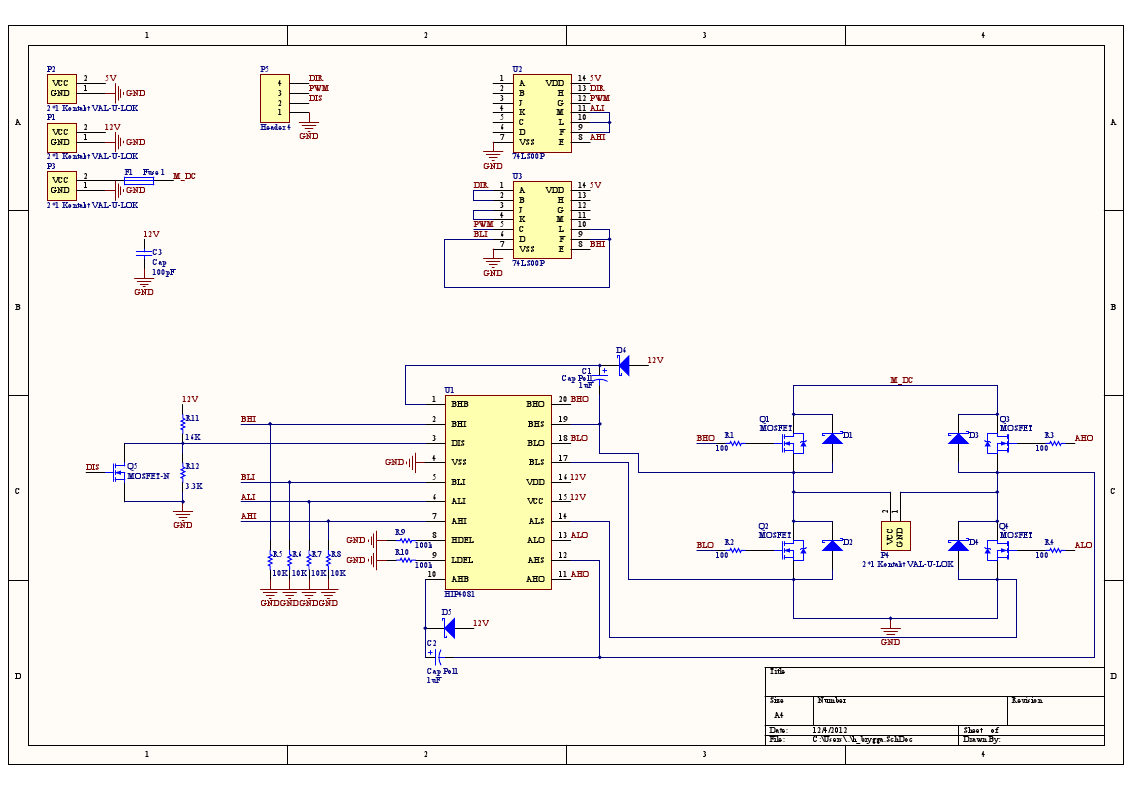
\includegraphics[width=18cm]{../../includes/figures/h_brygga_schematic}
\caption{H-bryggans kretsschema.}
\label{fig:appendix_h_brygga_schema}
\end{figure}
\end{landscape}

\begin{landscape}
\begin{figure}[htbp!]
\centering
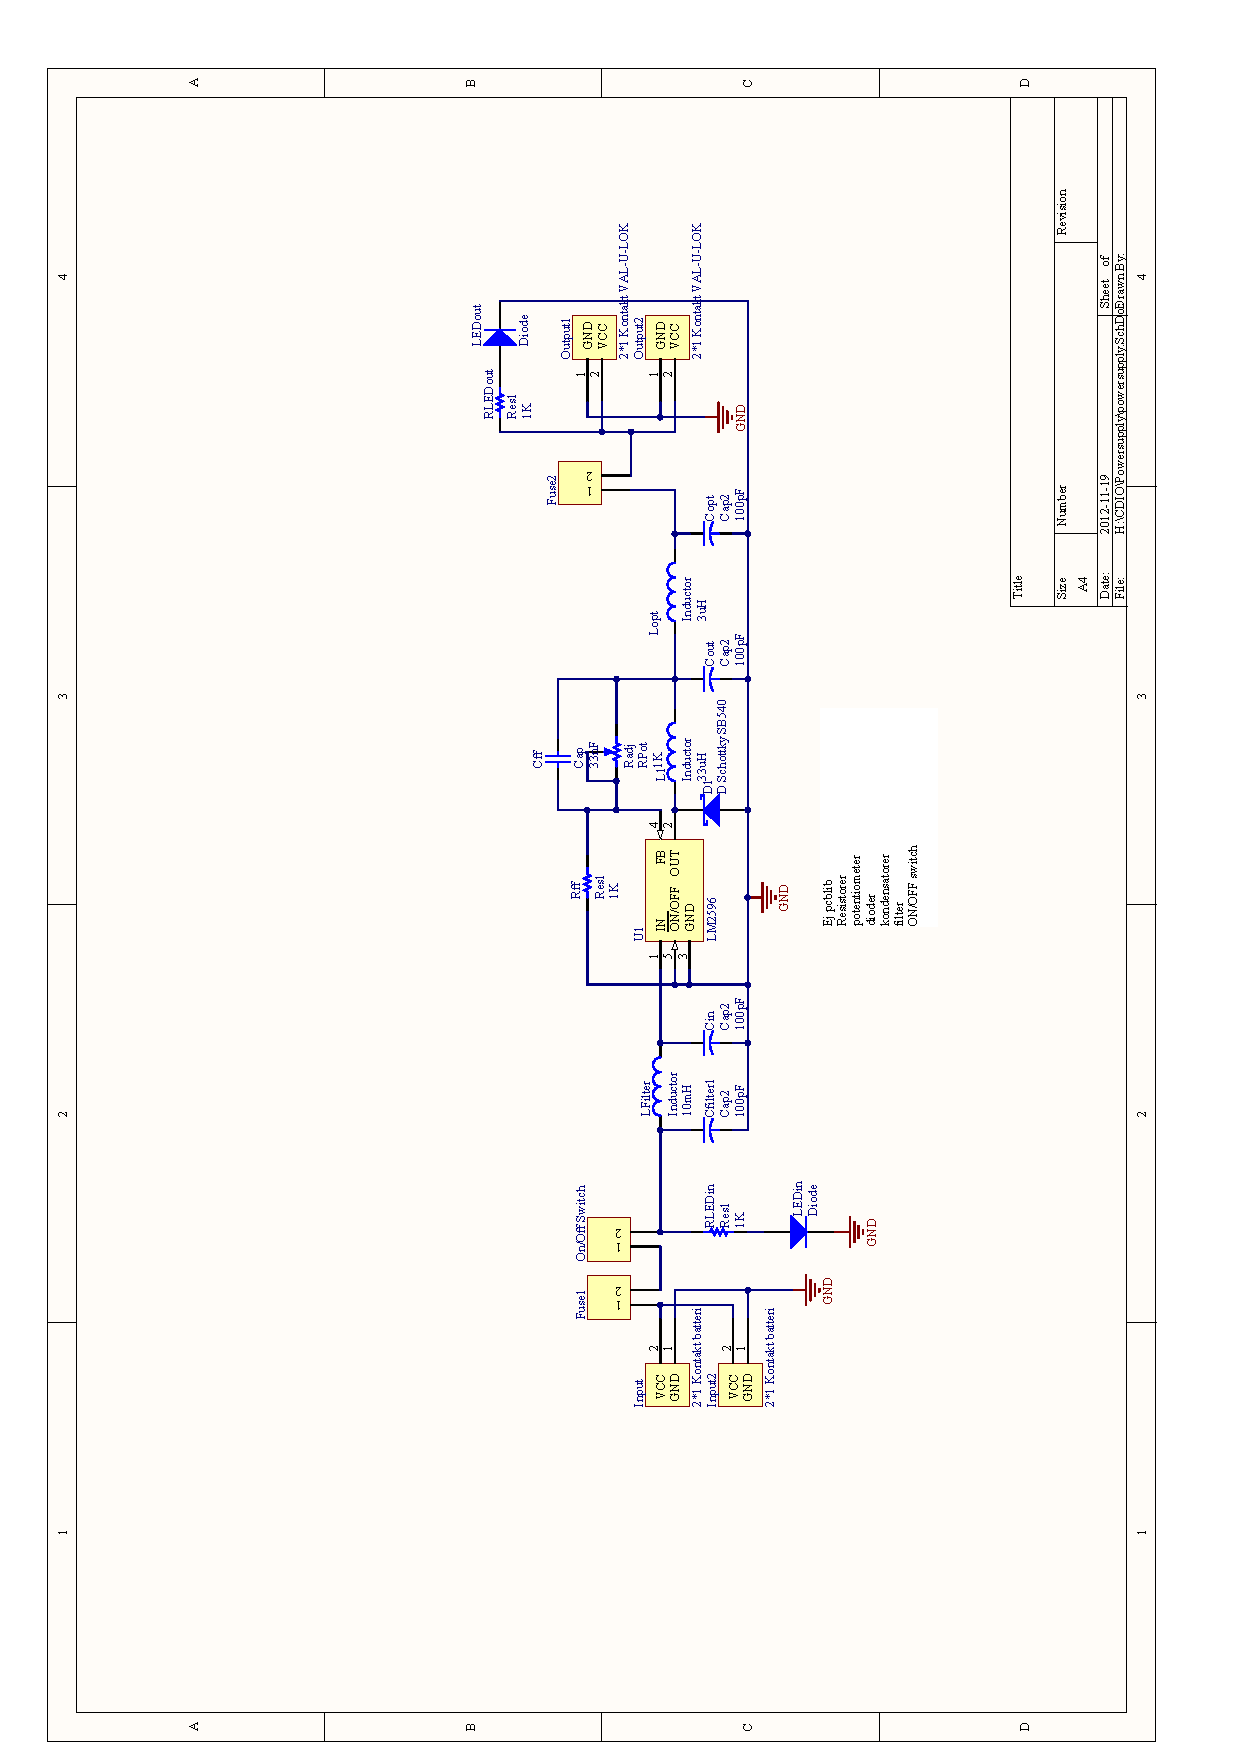
\includegraphics[height=18cm,angle=270]{../../includes/figures/PSU_Schematic}
\caption{Strömförsörjningens kretsschema.}
\label{fig:appendix_PSU_schema}
\end{figure}
\end{landscape}

\subsection{PCB-layout}
\begin{figure}[htbp!]
\centering
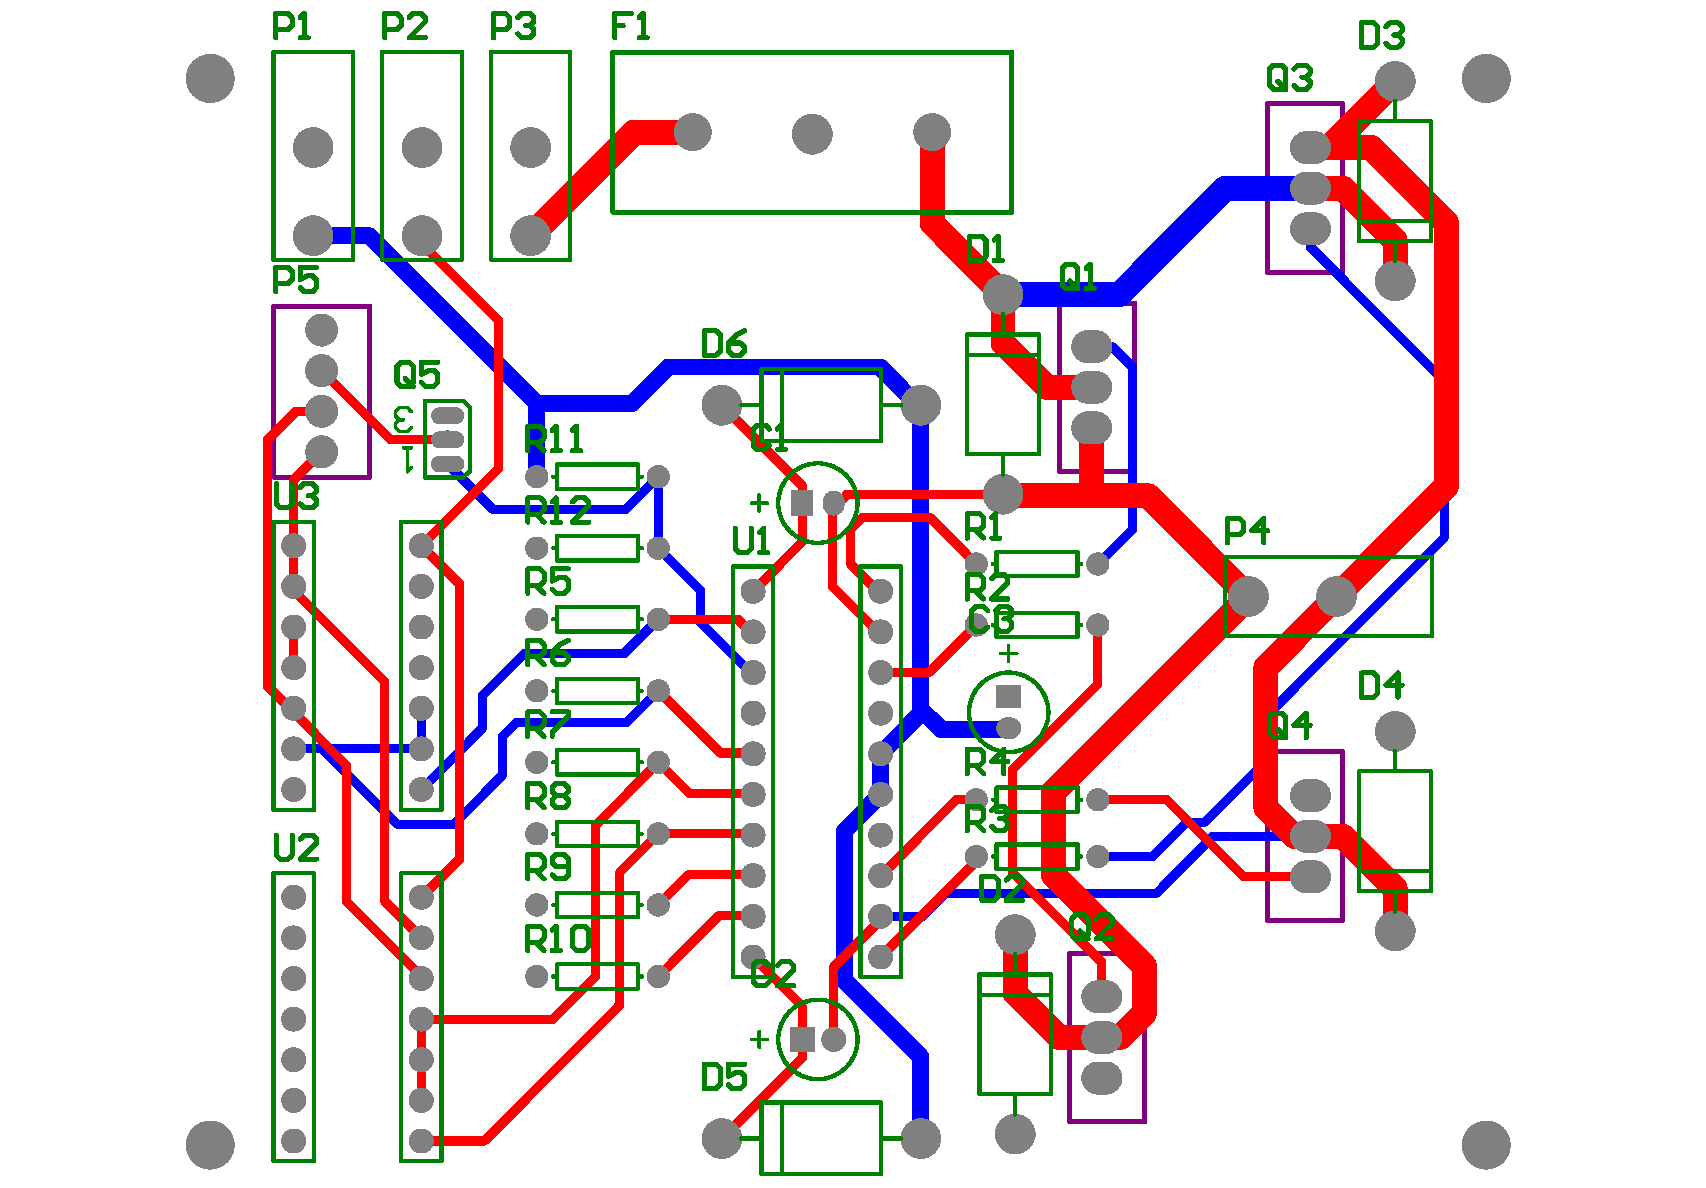
\includegraphics[width=12cm]{../../includes/figures/H_brygga_pcb}
\caption{H-bryggans PCB-layout.}
\label{fig:appendix_pcb_layout}
\end{figure}

\begin{figure}[htbp!]
\centering
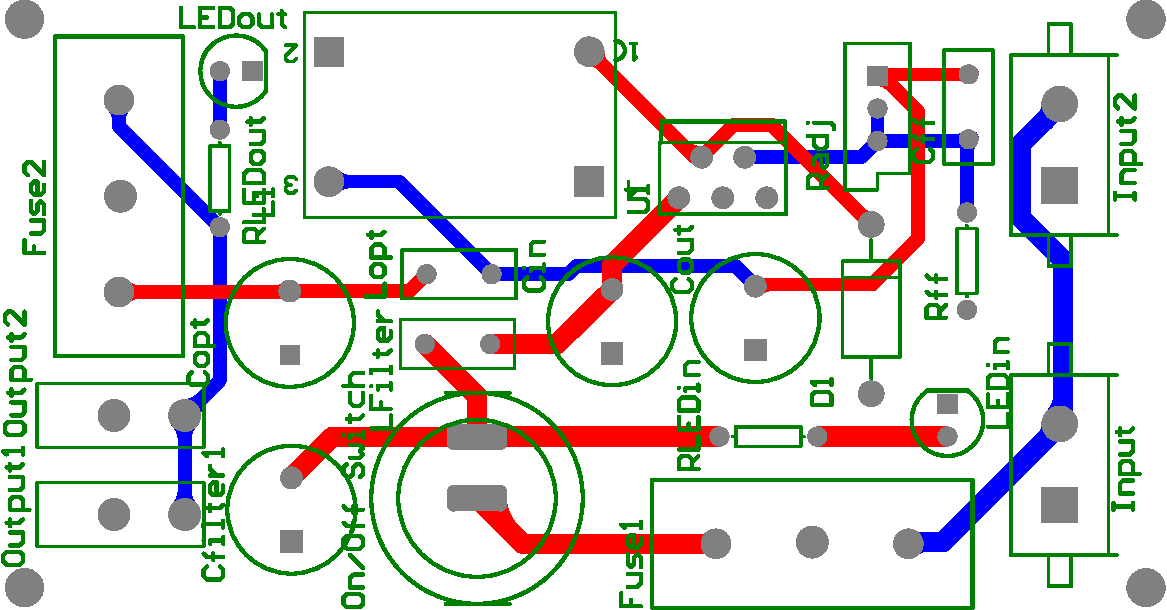
\includegraphics[width=12cm,angle=270]{../../includes/figures/PSU_PCB}
\caption{Strömförsörjningens PCB-layout.}
\label{fig:appendix_PSU_pcb_layout}
\end{figure}

\section{Chassi}
\begin{landscape}
\begin{figure}[htbp!]
\centering
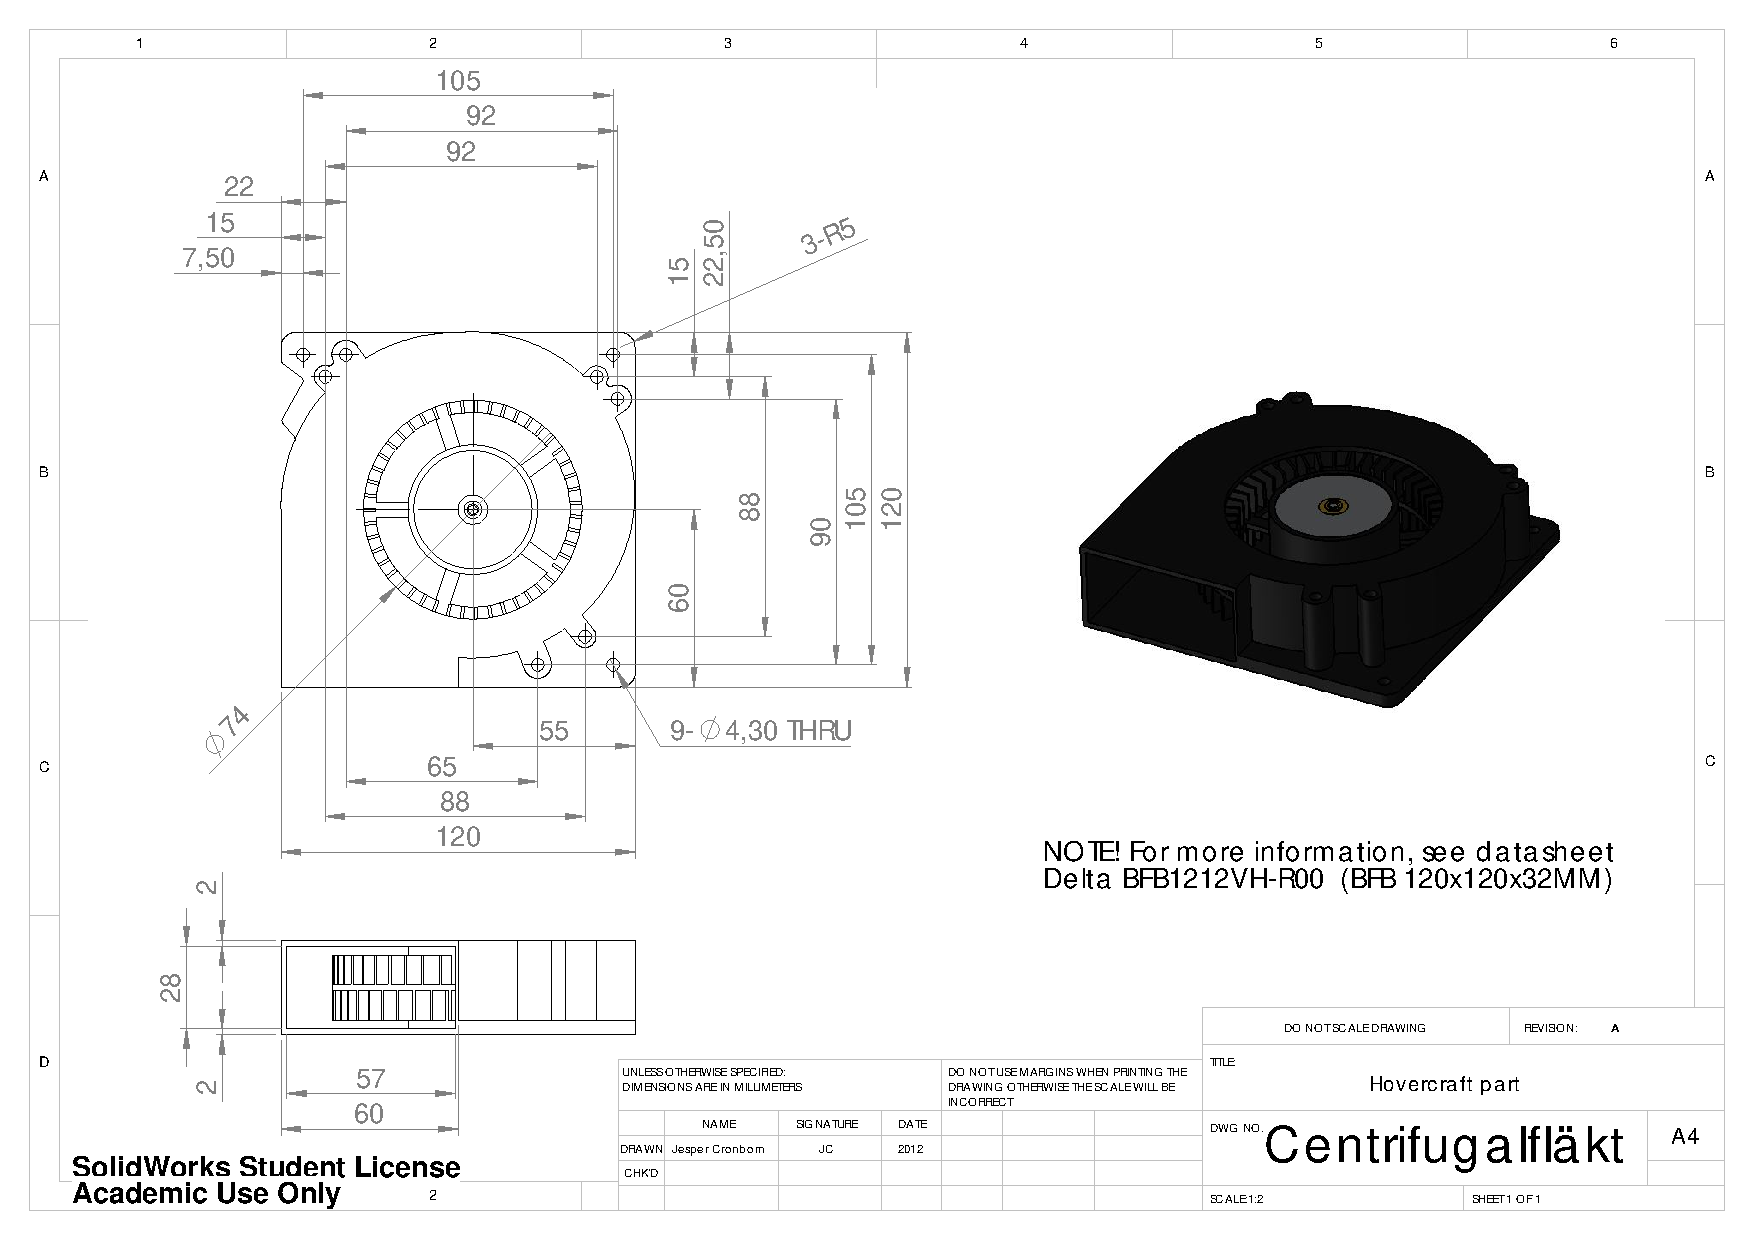
\includegraphics[width=18cm]{../../includes/figures/PDF_ritningar/Centrifugalflakt}
\caption{Ritning över centrifugalfläkt.}
\label{fig:Centrifugalfläkt}
\end{figure}
\end{landscape}

\begin{landscape}
\begin{figure}[htbp!]
\centering
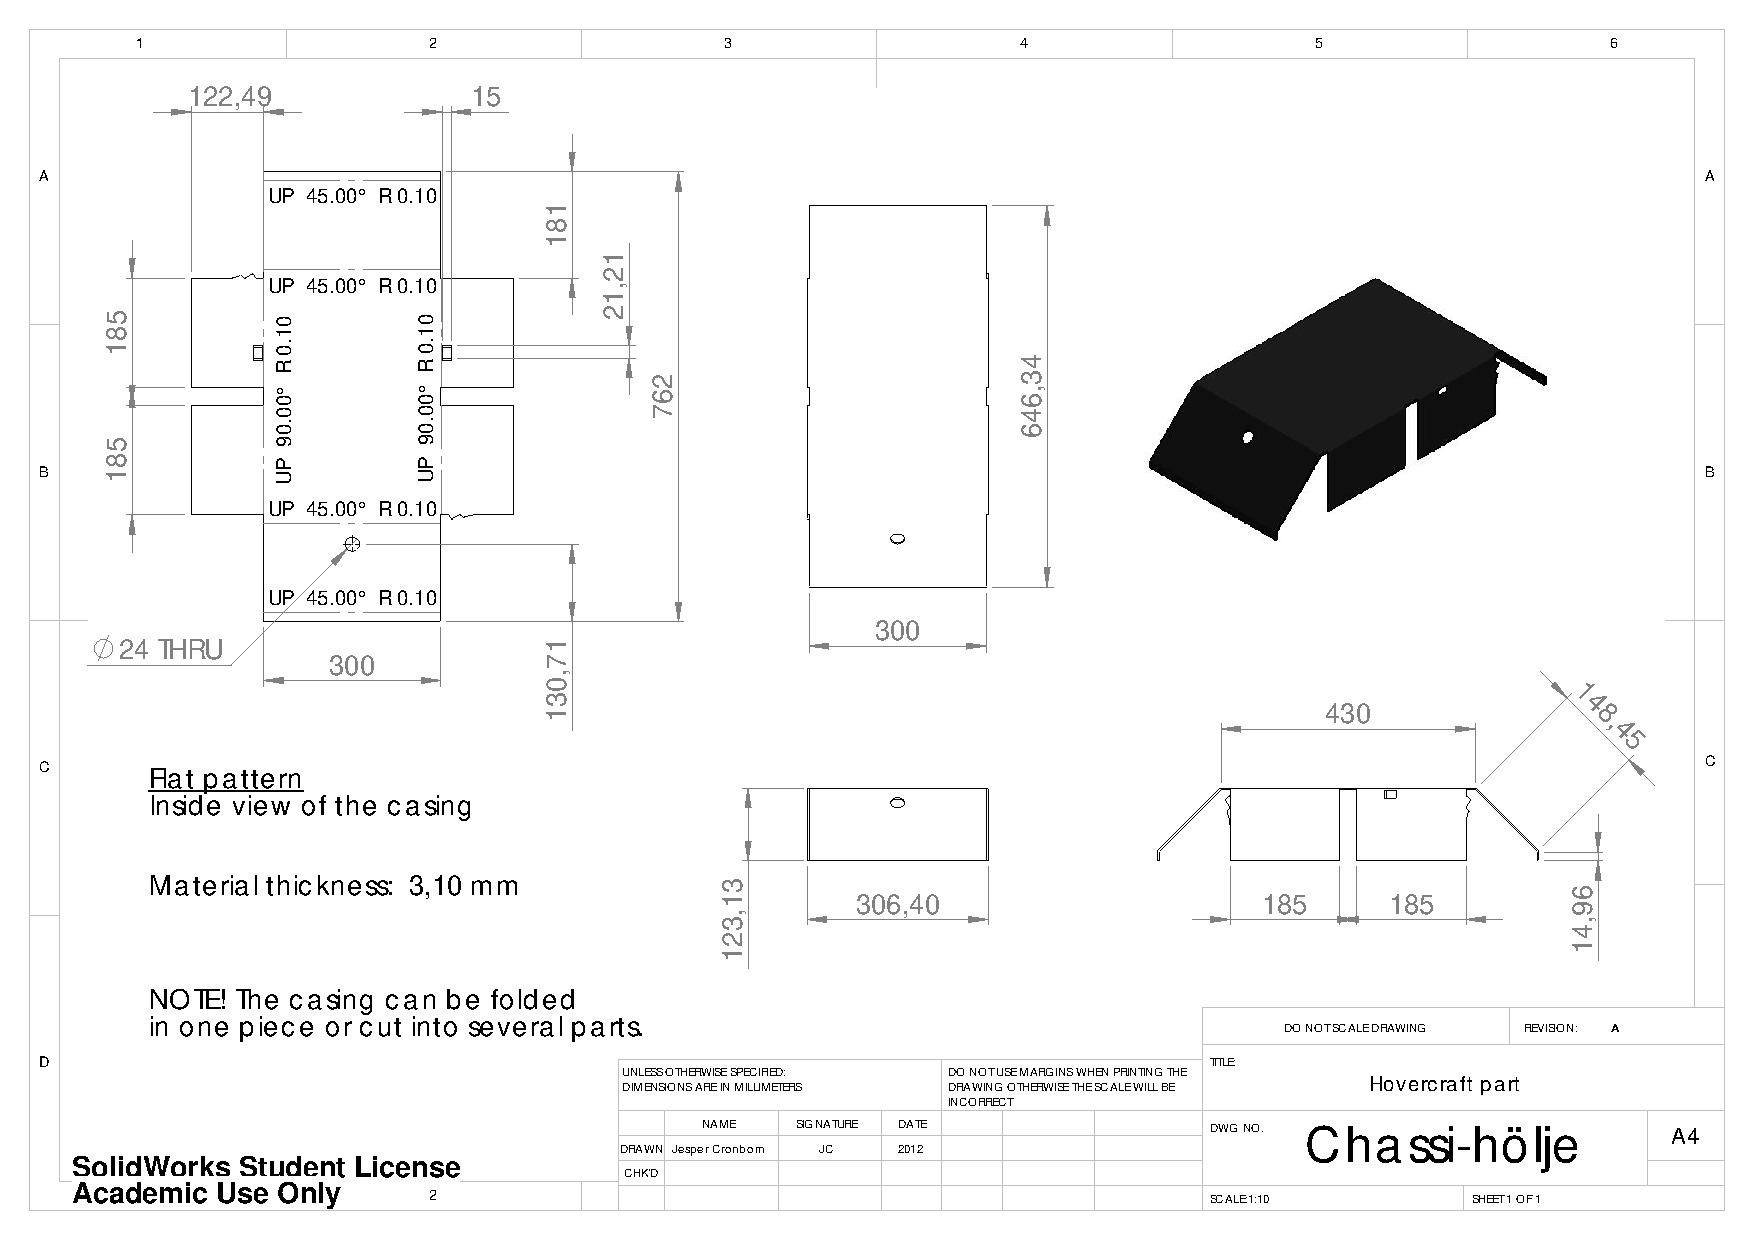
\includegraphics[width=18cm]{../../includes/figures/PDF_ritningar/Chassi_holje}
\caption{Ritning över Chassi hölje.}
\label{fig:Chassi_holje}
\end{figure}
\end{landscape}

\begin{landscape}
\begin{figure}[htbp!]
\centering
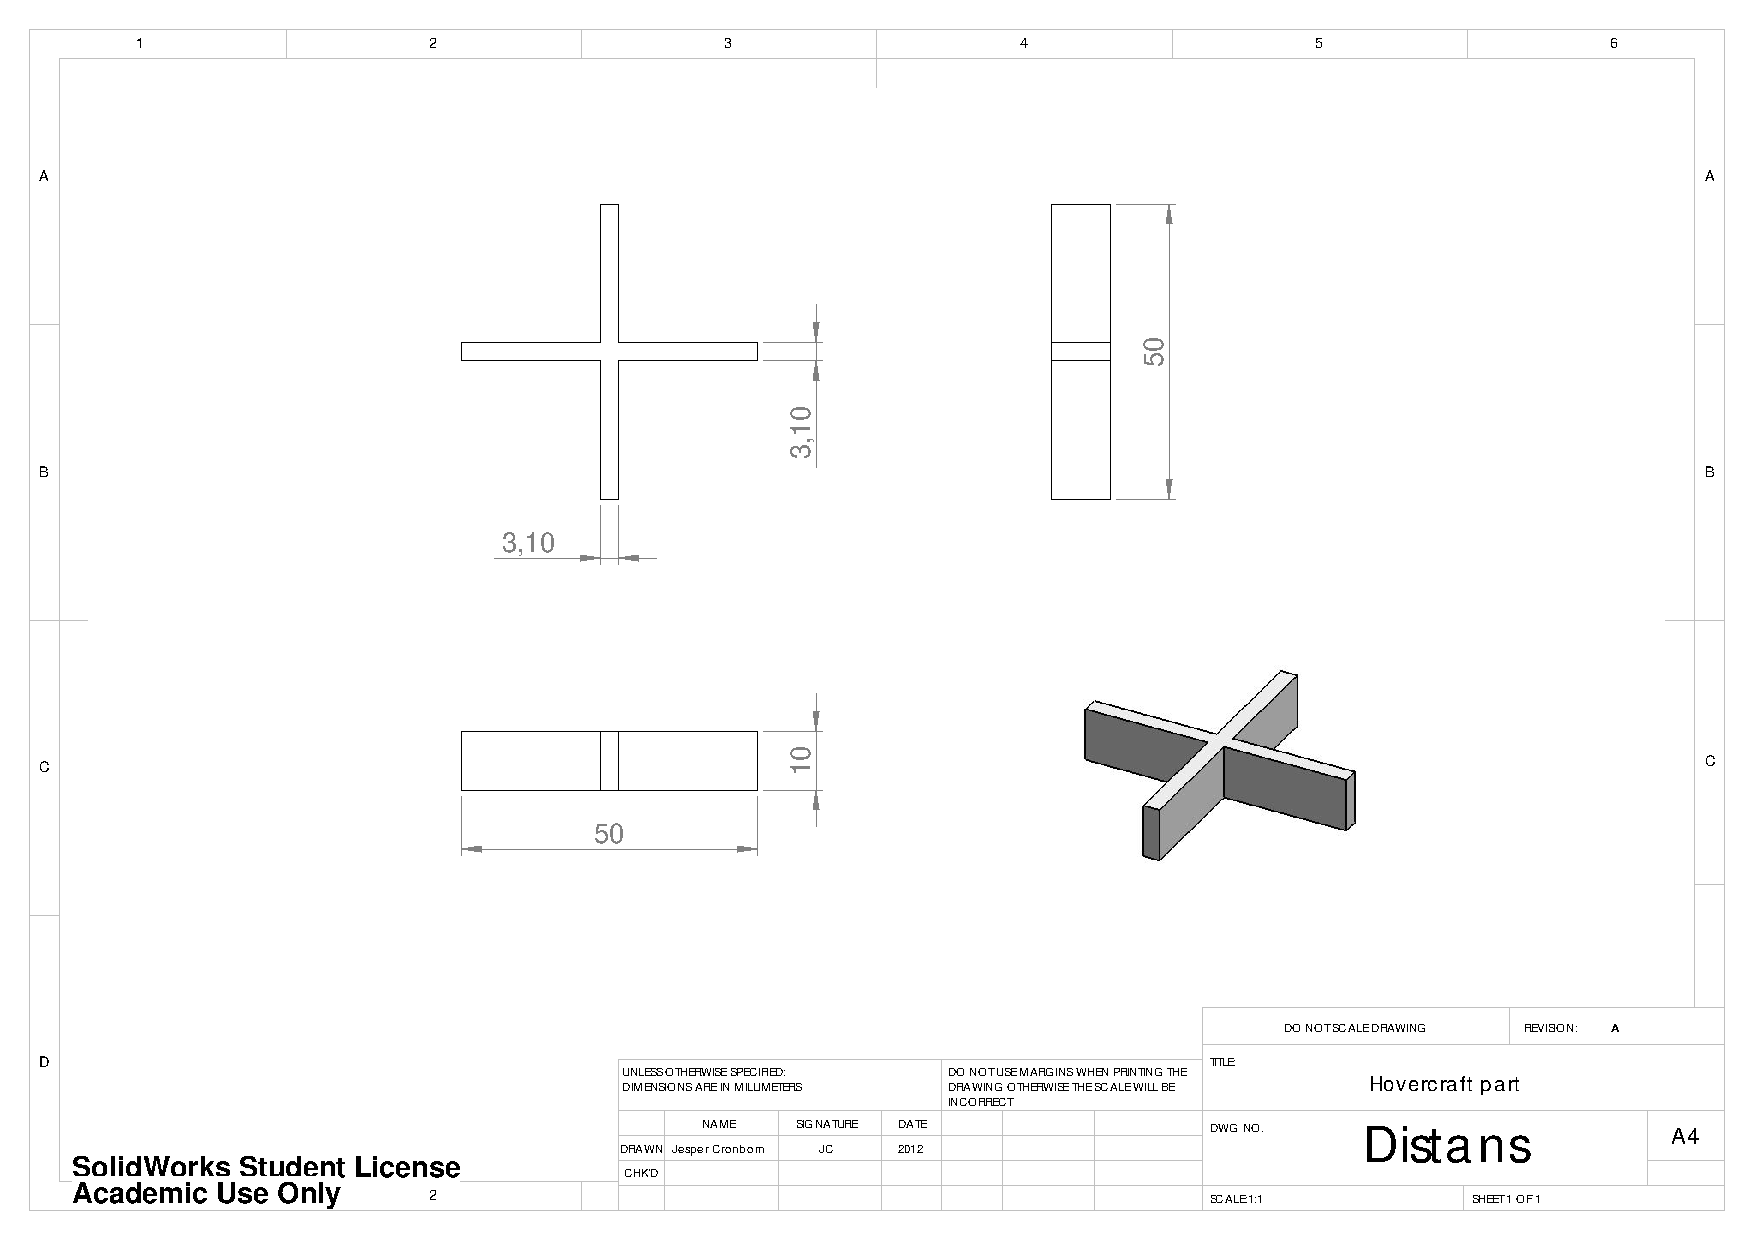
\includegraphics[width=18cm]{../../includes/figures/PDF_ritningar/Distans}
\caption{Ritning över distans.}
\label{fig:Distans}
\end{figure}
\end{landscape}

\begin{landscape}
\begin{figure}[htbp!]
\centering
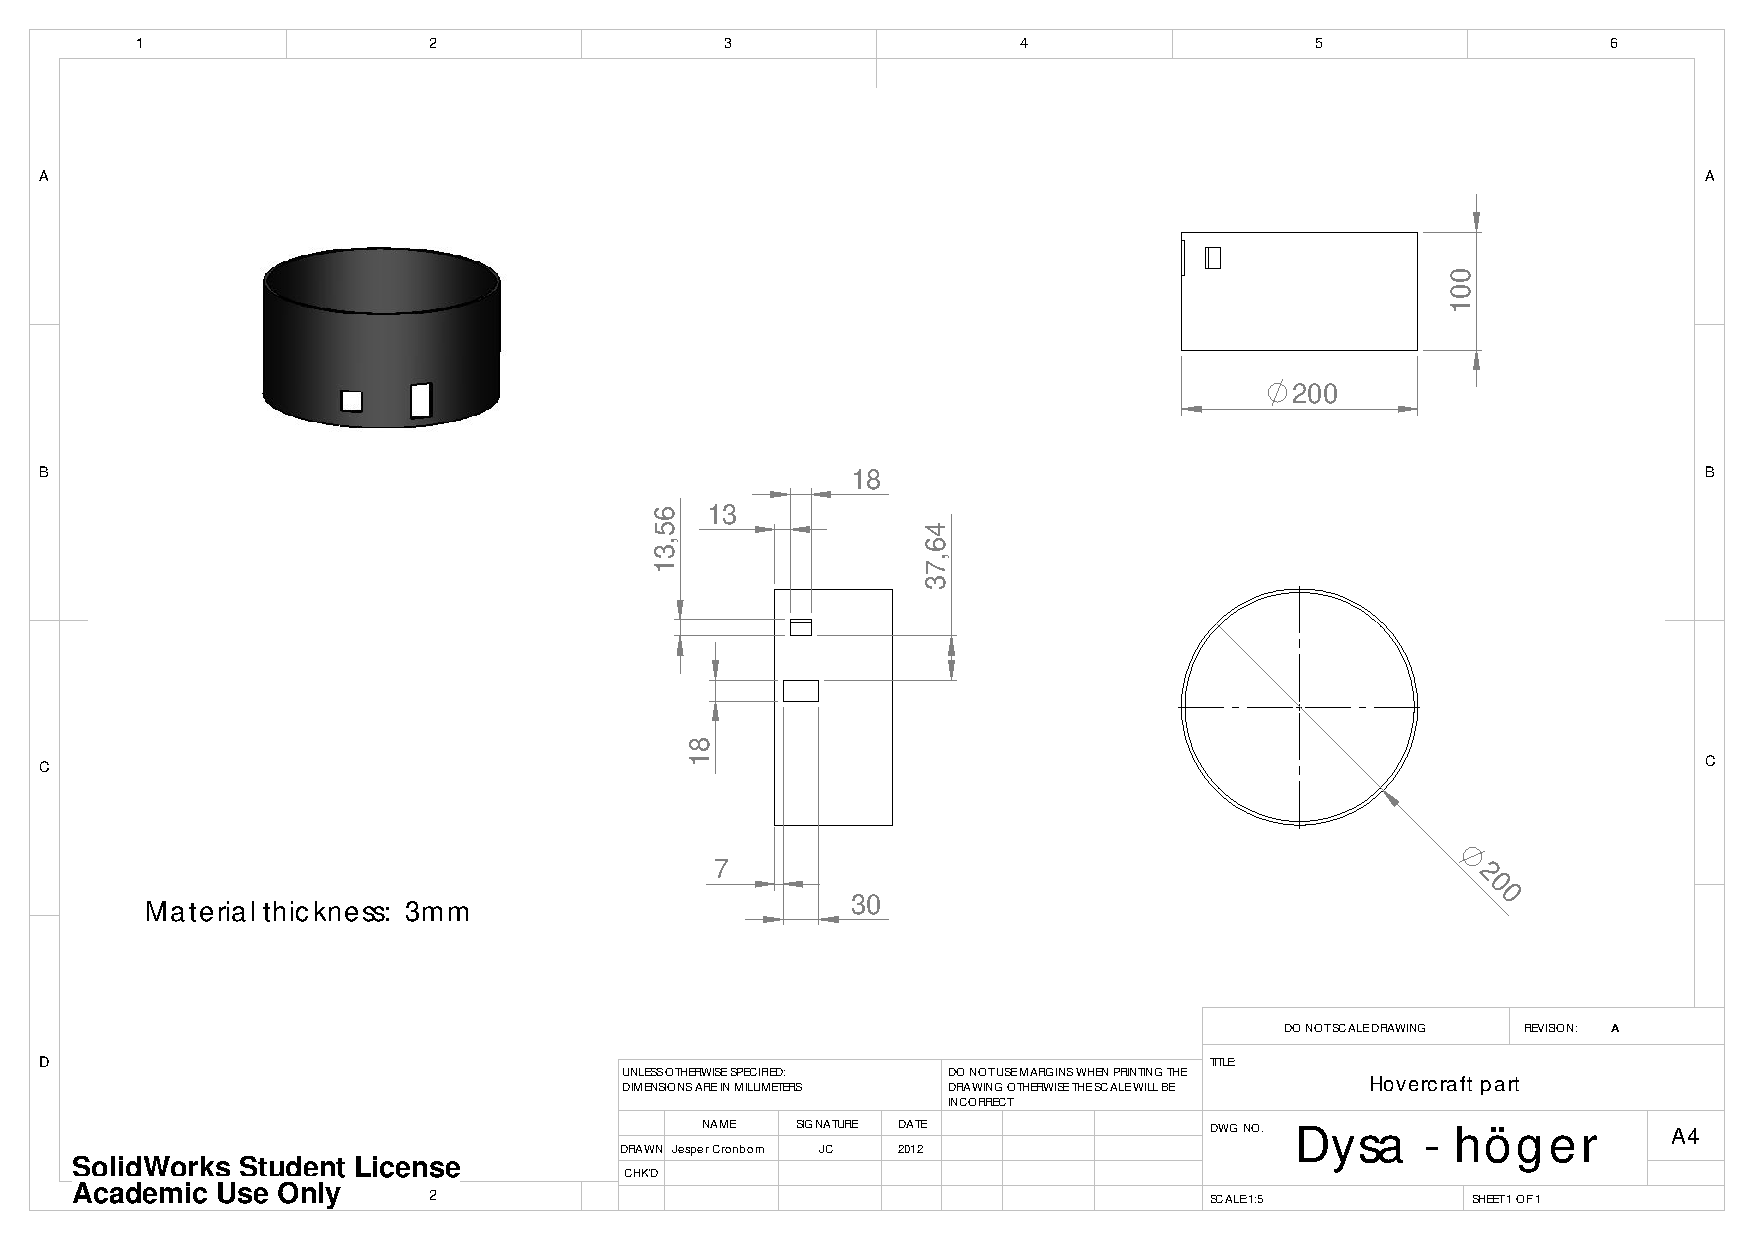
\includegraphics[width=18cm]{../../includes/figures/PDF_ritningar/Dysa_hoger}
\caption{Ritning över höger dysa.}
\label{fig:Dysa-höger}
\end{figure}
\end{landscape}

\begin{landscape}
\begin{figure}[htbp!]
\centering
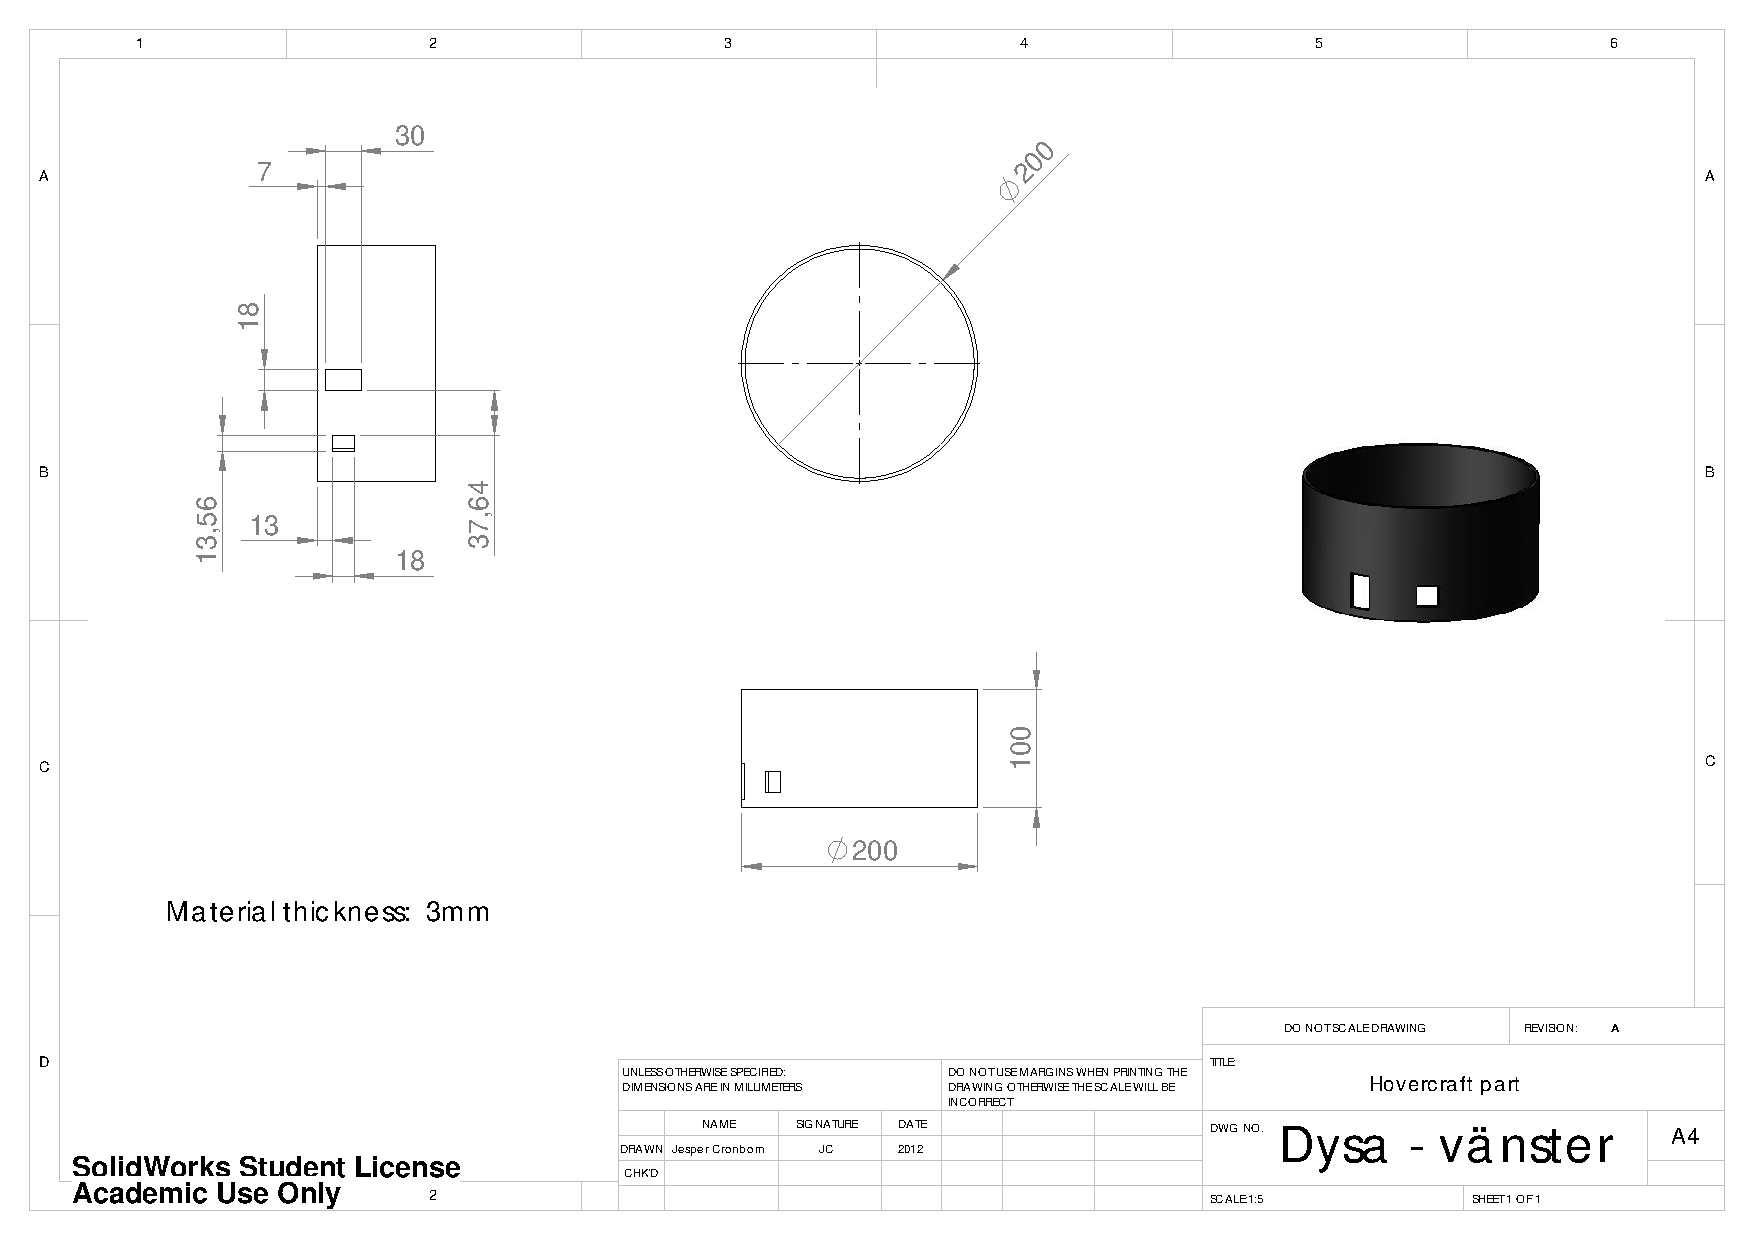
\includegraphics[width=18cm]{../../includes/figures/PDF_ritningar/Dysa_vanster}
\caption{Ritning över vänster dysa.}
\label{fig:Dysa-höger}
\end{figure}
\end{landscape}

\begin{landscape}
\begin{figure}[htbp!]
\centering
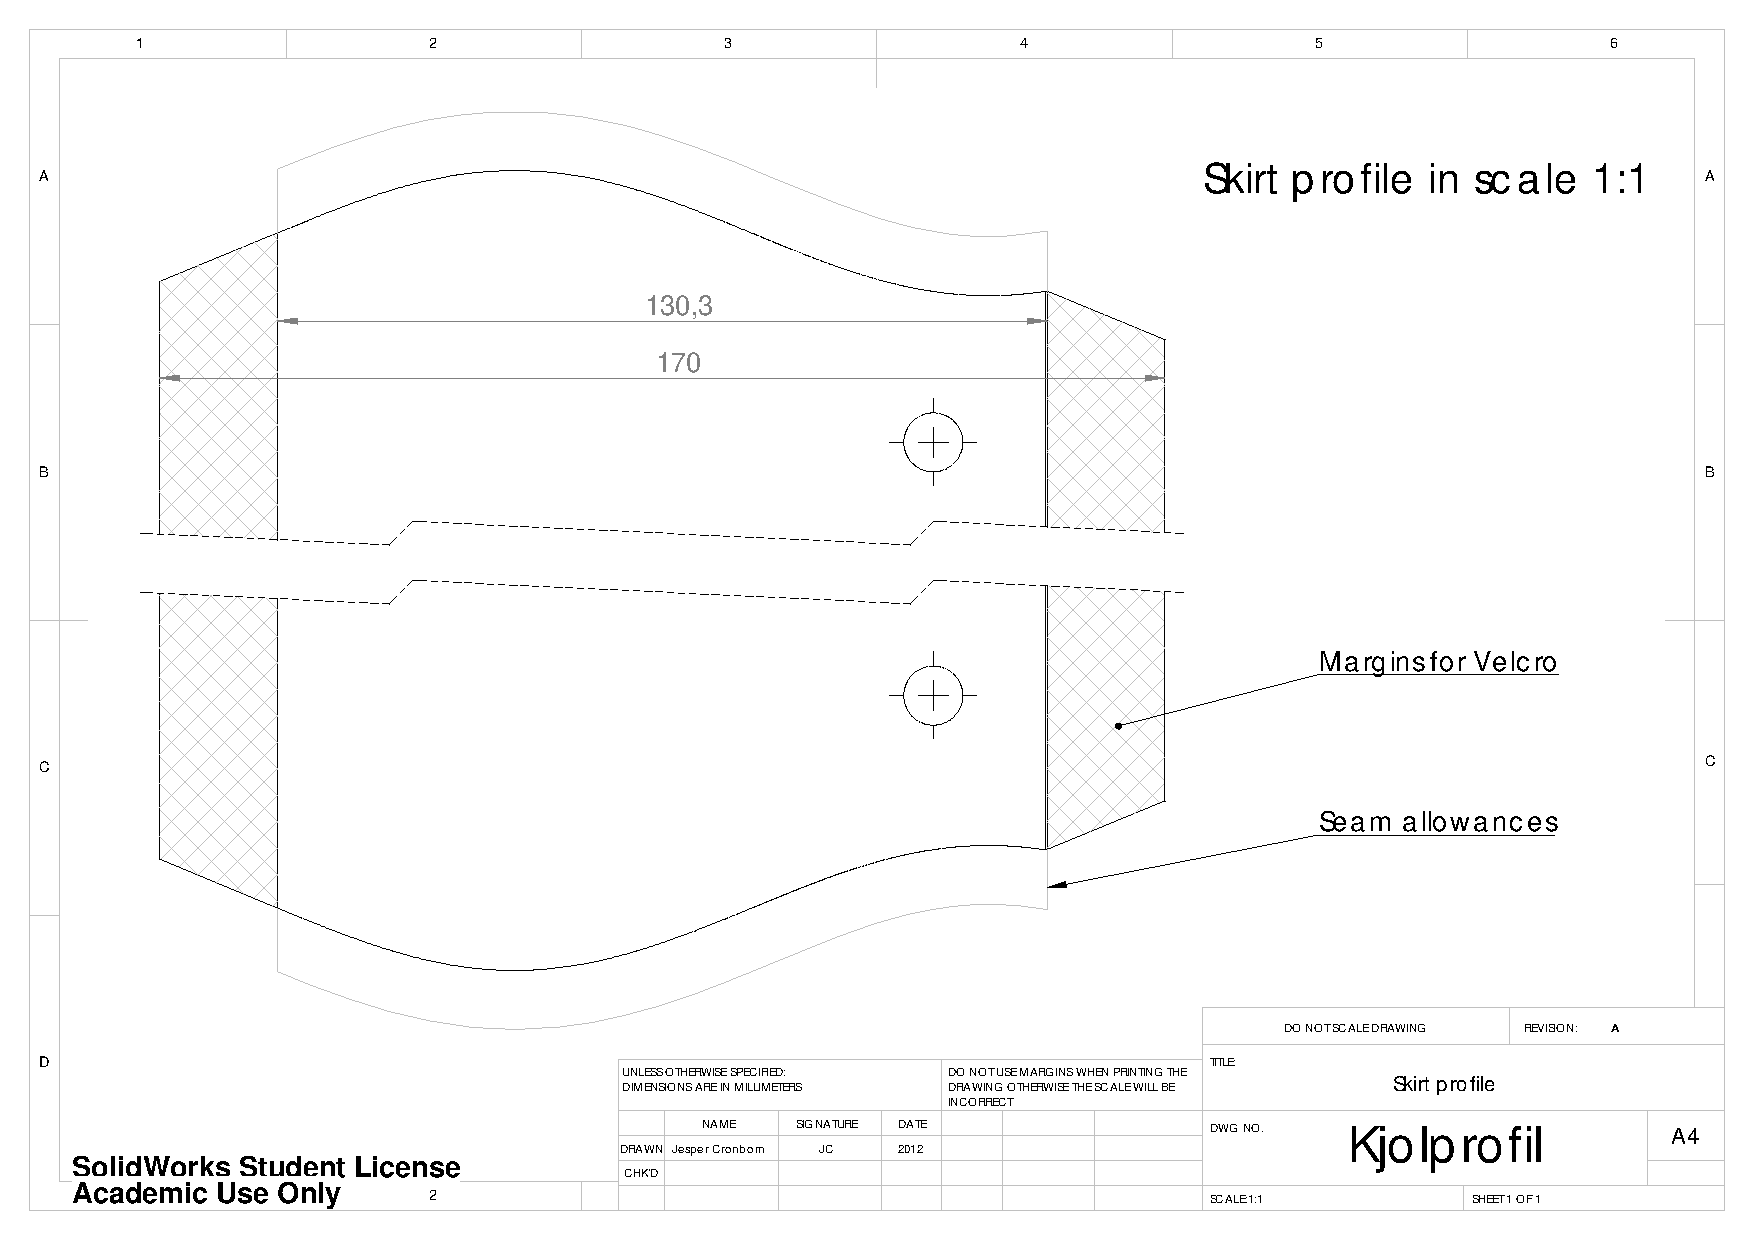
\includegraphics[width=18cm]{../../includes/figures/PDF_ritningar/Kjolprofil}
\caption{Ritning över kjolprofil.}
\label{fig:Kjolprofil}
\end{figure}
\end{landscape}

\begin{landscape}
\begin{figure}[htbp!]
\centering
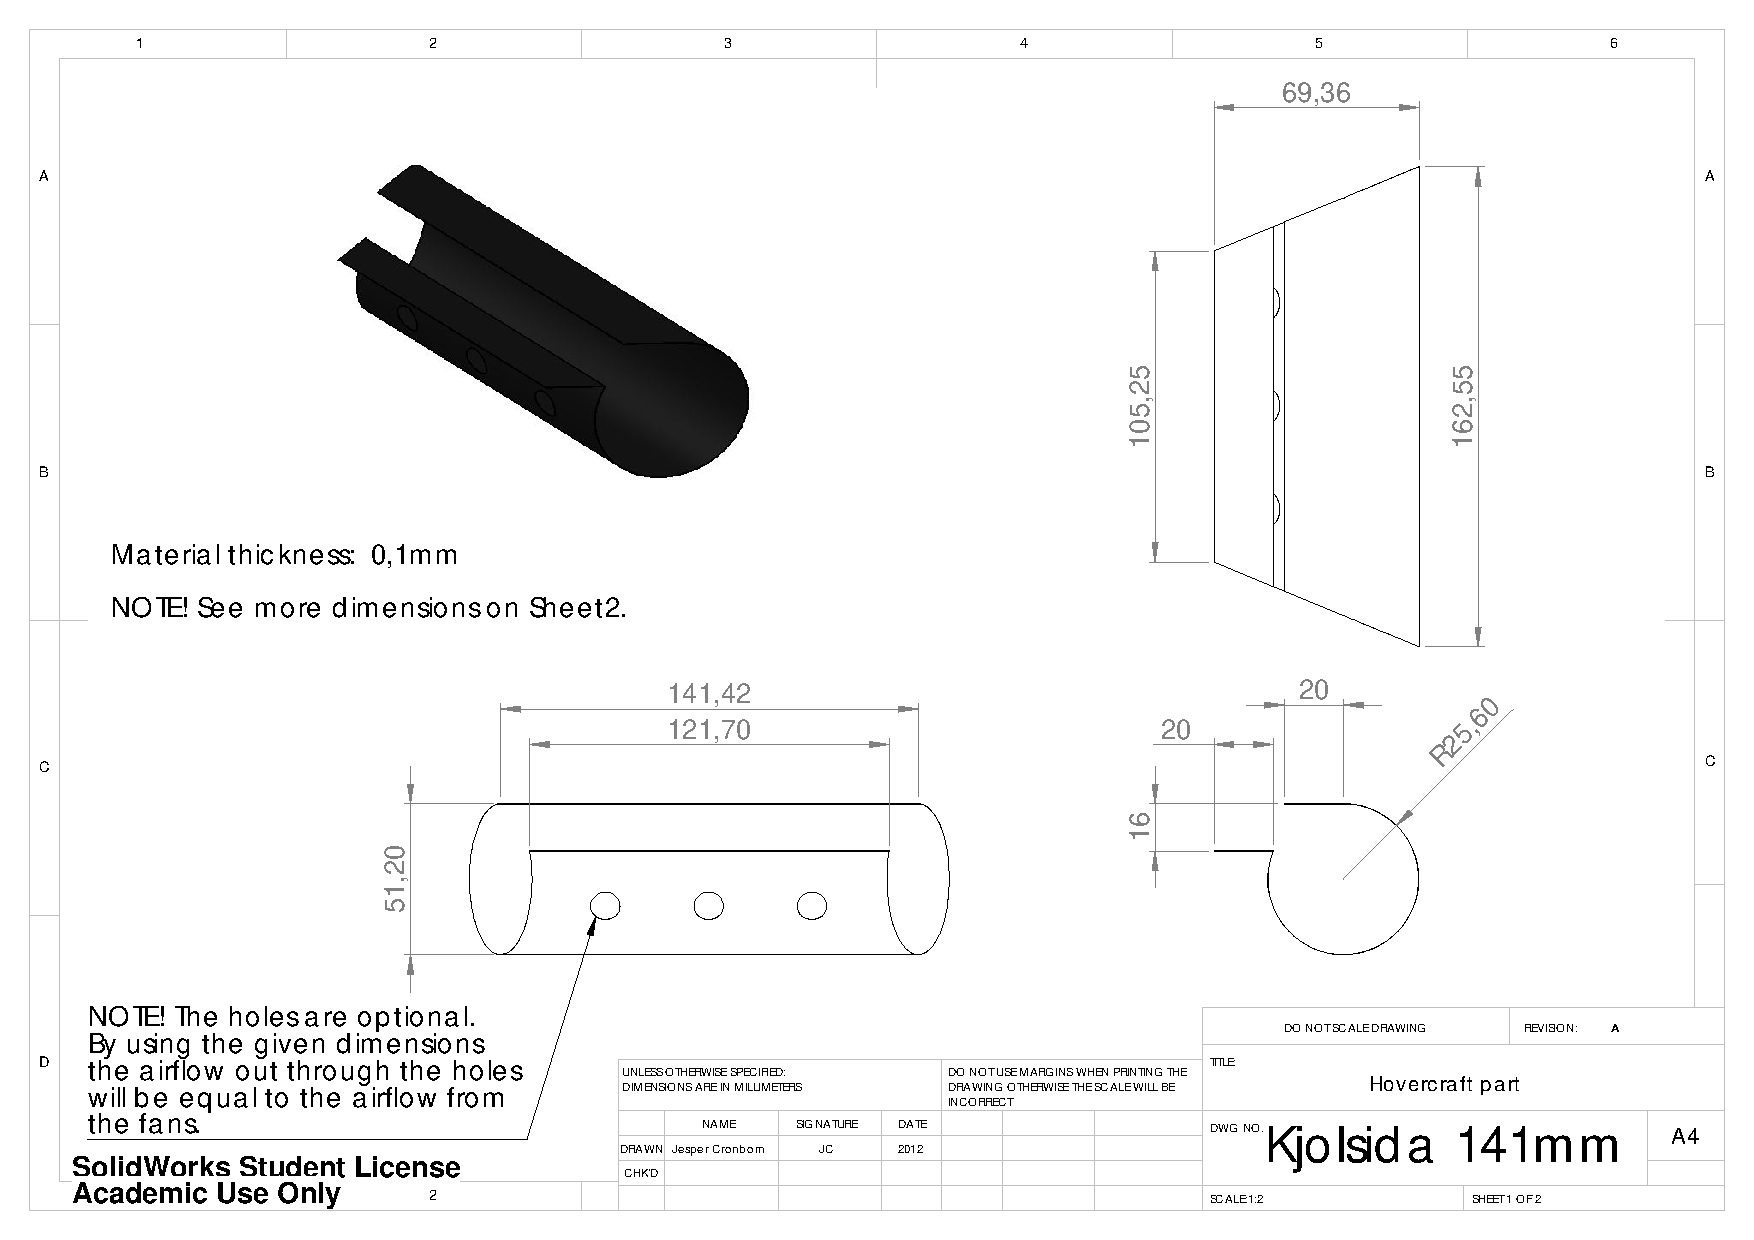
\includegraphics[width=18cm]{../../includes/figures/PDF_ritningar/Kjolsida_141}
\caption{Ritning över kjolsida 141.}
\label{fig:kjolsida141}
\end{figure}
\end{landscape}

\begin{landscape}
\begin{figure}[htbp!]
\centering
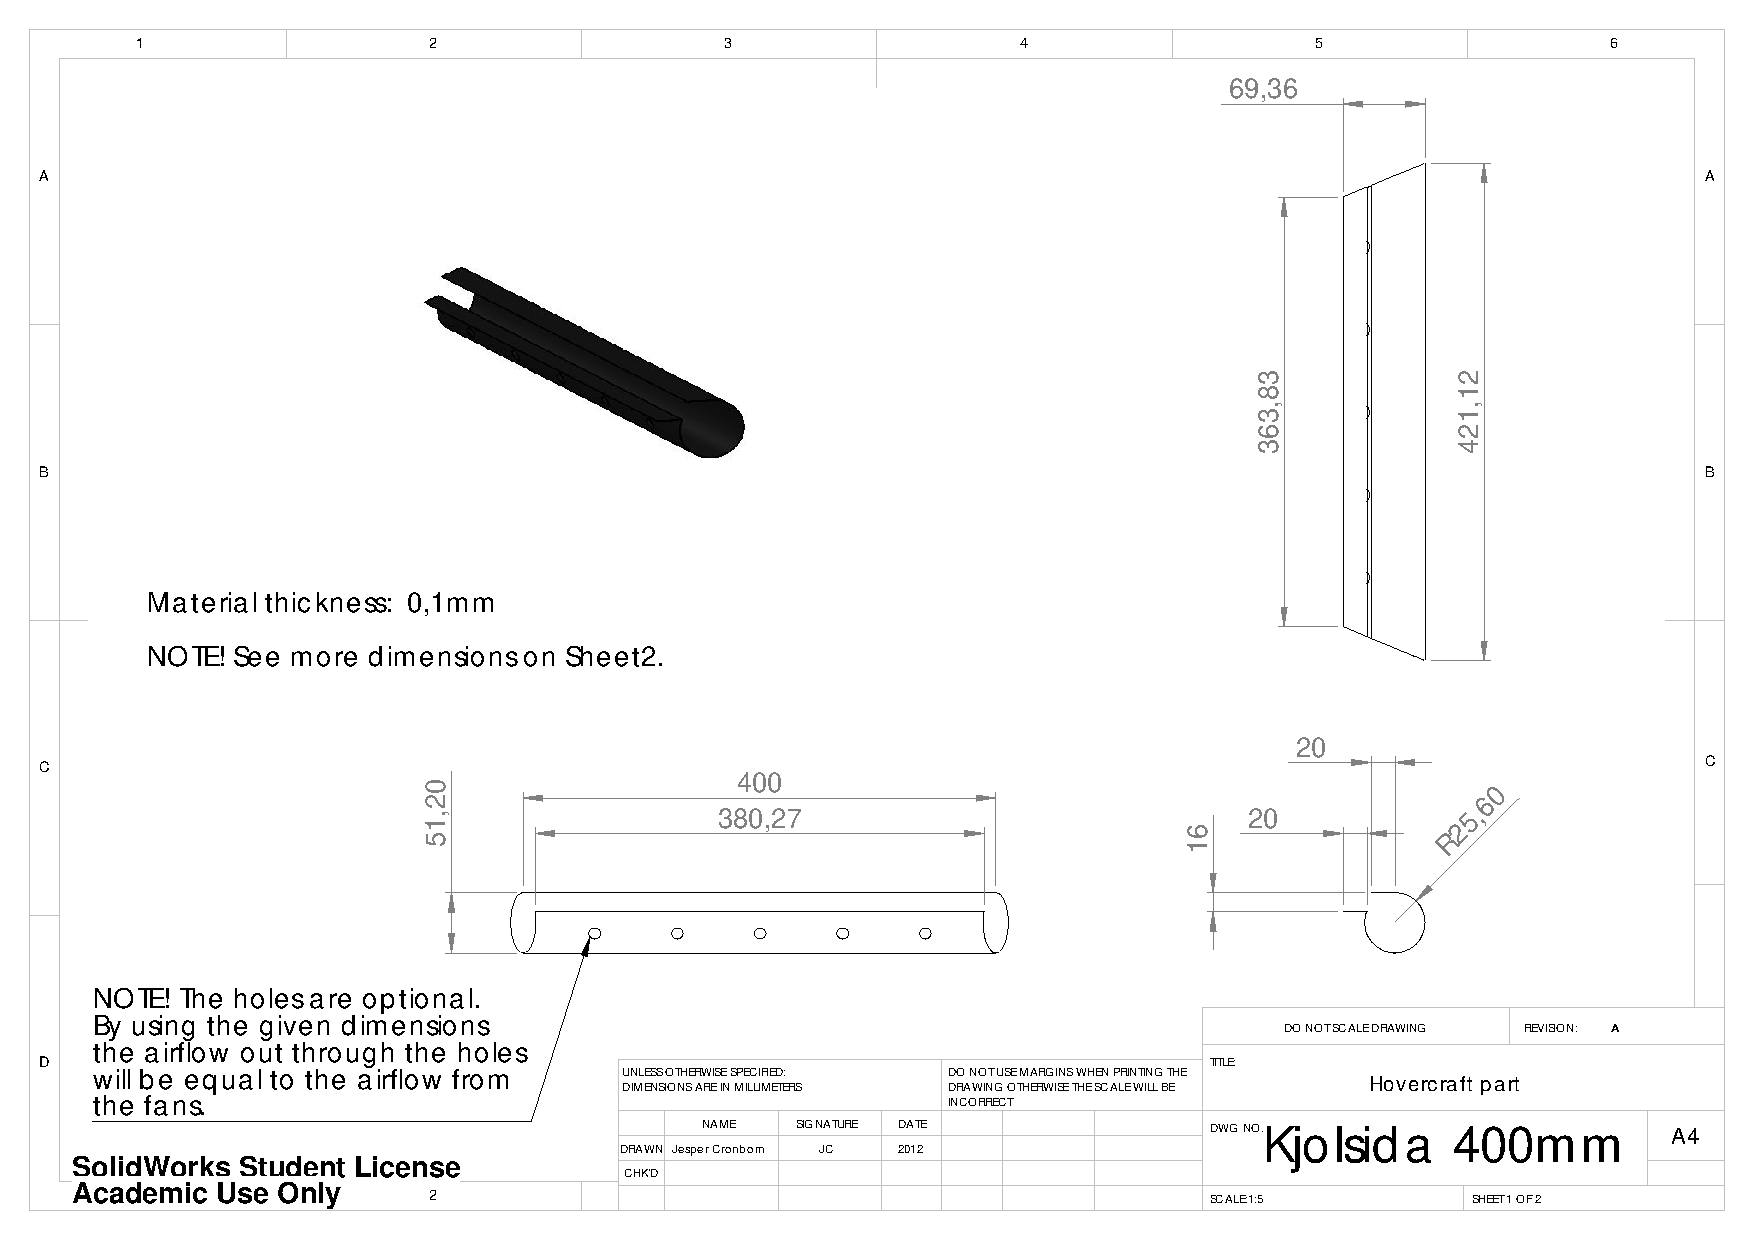
\includegraphics[width=18cm]{../../includes/figures/PDF_ritningar/Kjolsida_400}
\caption{Ritning över Kjolsida 400.}
\label{fig:Kjolsida_400}
\end{figure}
\end{landscape}

\begin{landscape}
\begin{figure}[htbp!]
\centering
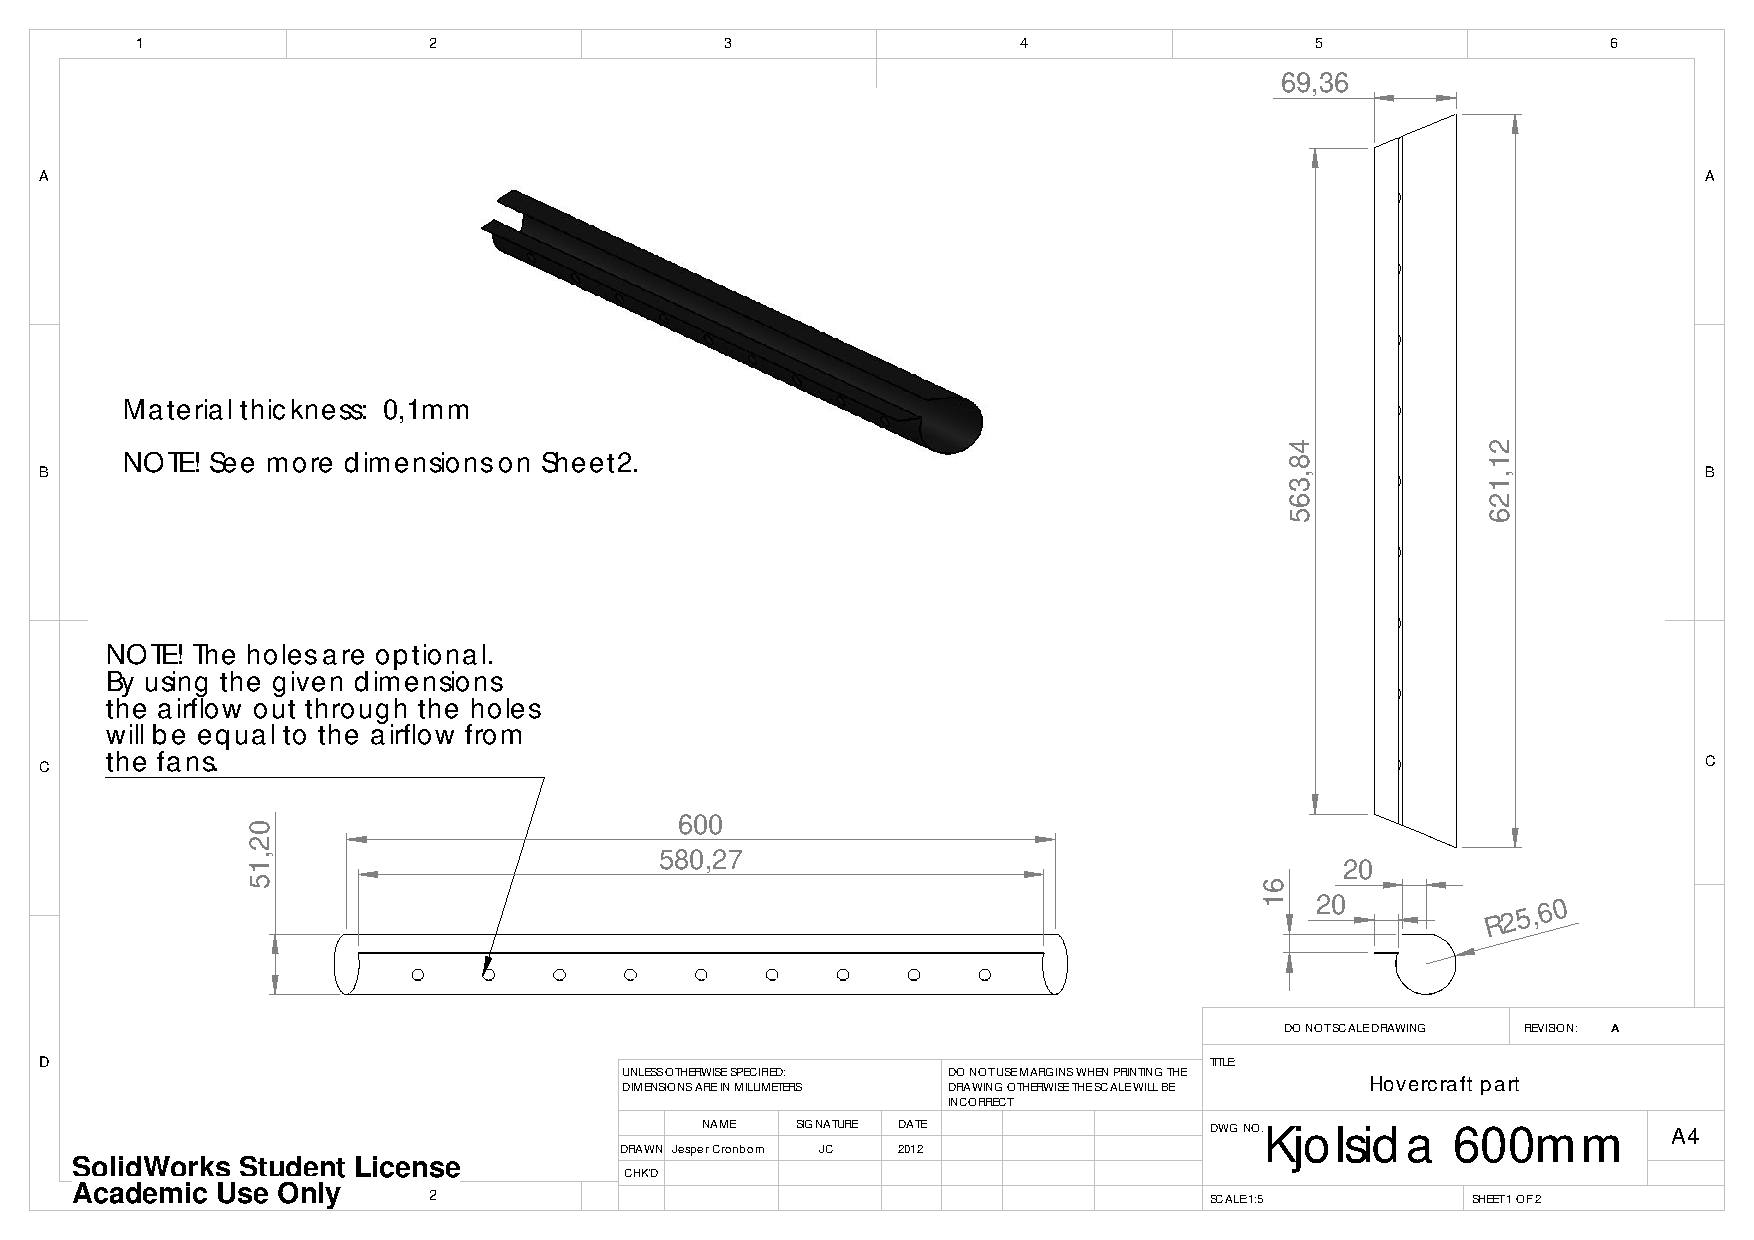
\includegraphics[width=18cm]{../../includes/figures/PDF_ritningar/Kjolsida_600}
\caption{Ritning över Kjolsida 600.}
\label{fig:Kjolsida_600}
\end{figure}
\end{landscape}

\begin{landscape}
\begin{figure}[htbp!]
\centering
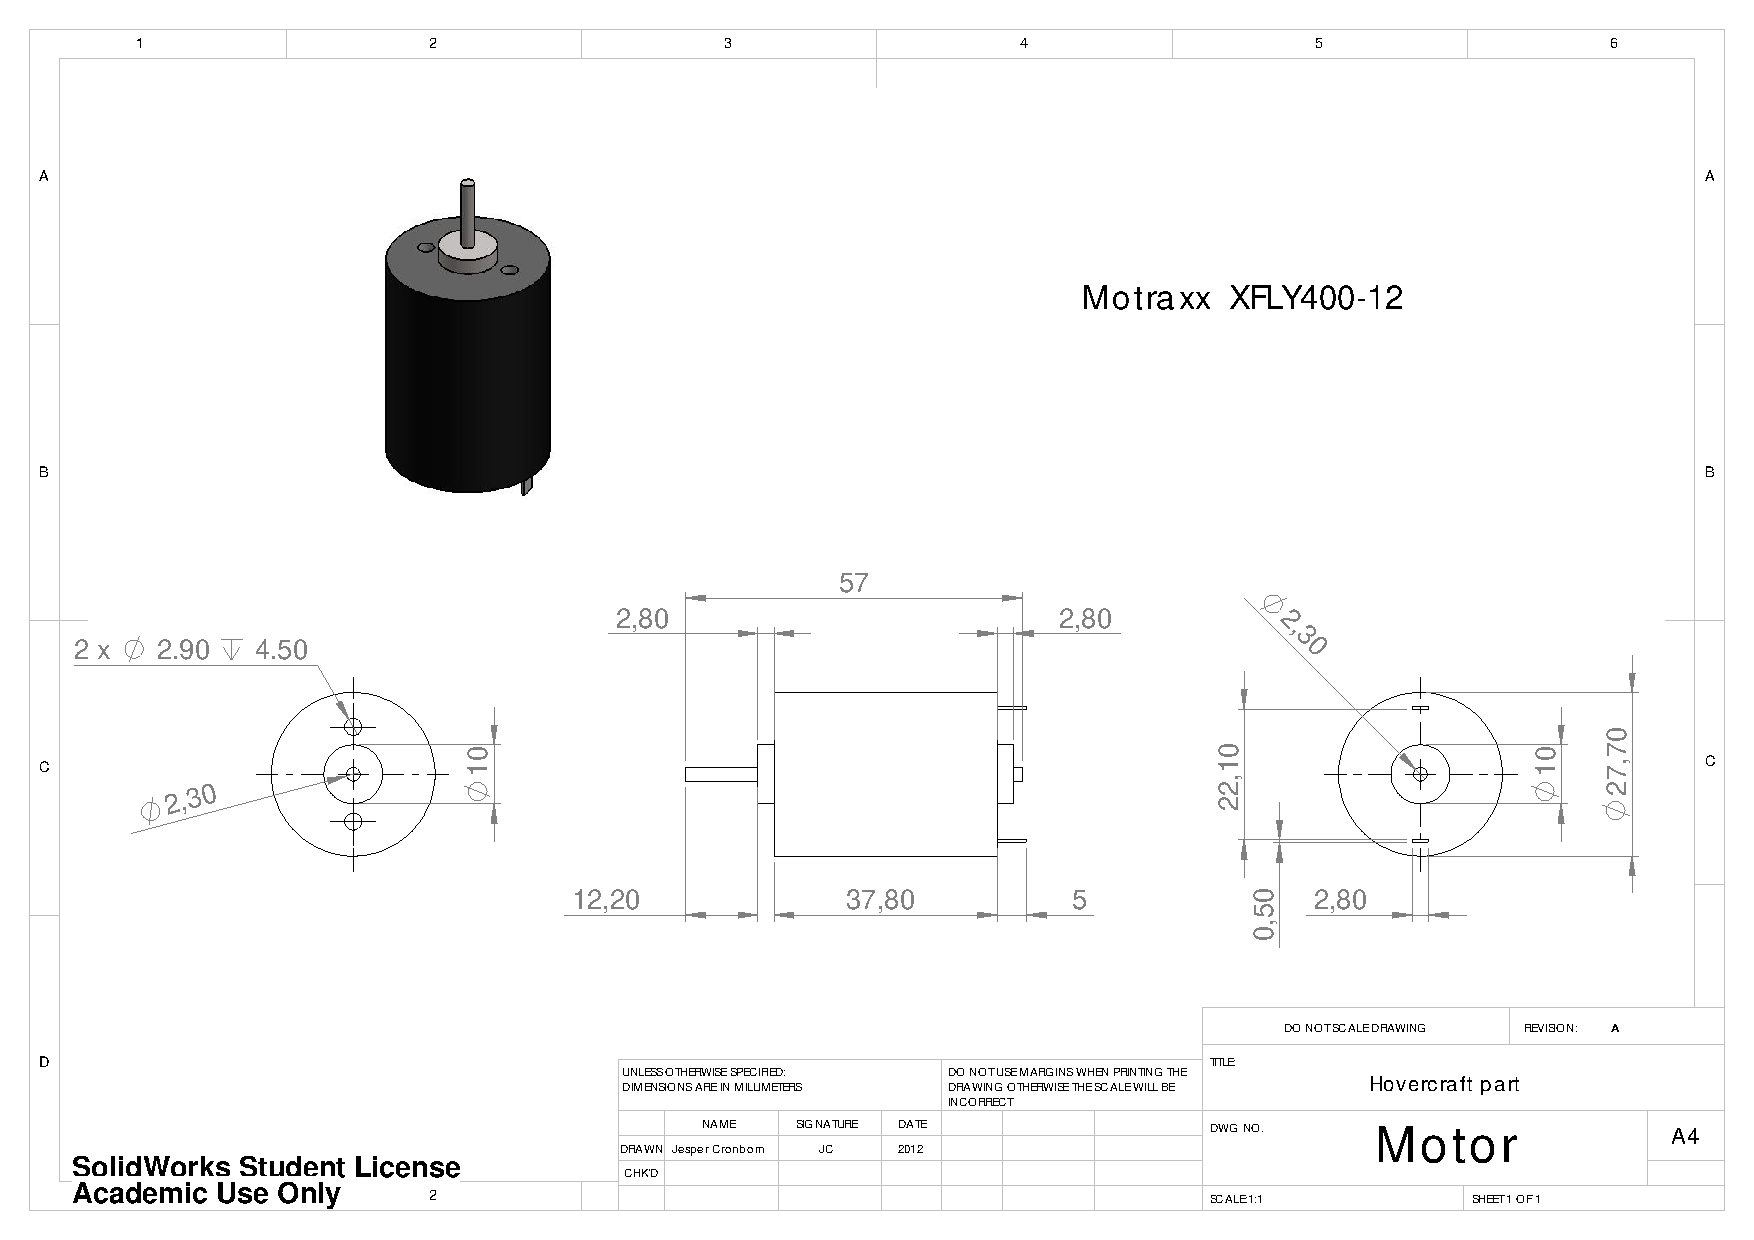
\includegraphics[width=18cm]{../../includes/figures/PDF_ritningar/Motor}
\caption{Ritning över motor.}
\label{fig:motor}
\end{figure}
\end{landscape}

\begin{landscape}
\begin{figure}[htbp!]
\centering
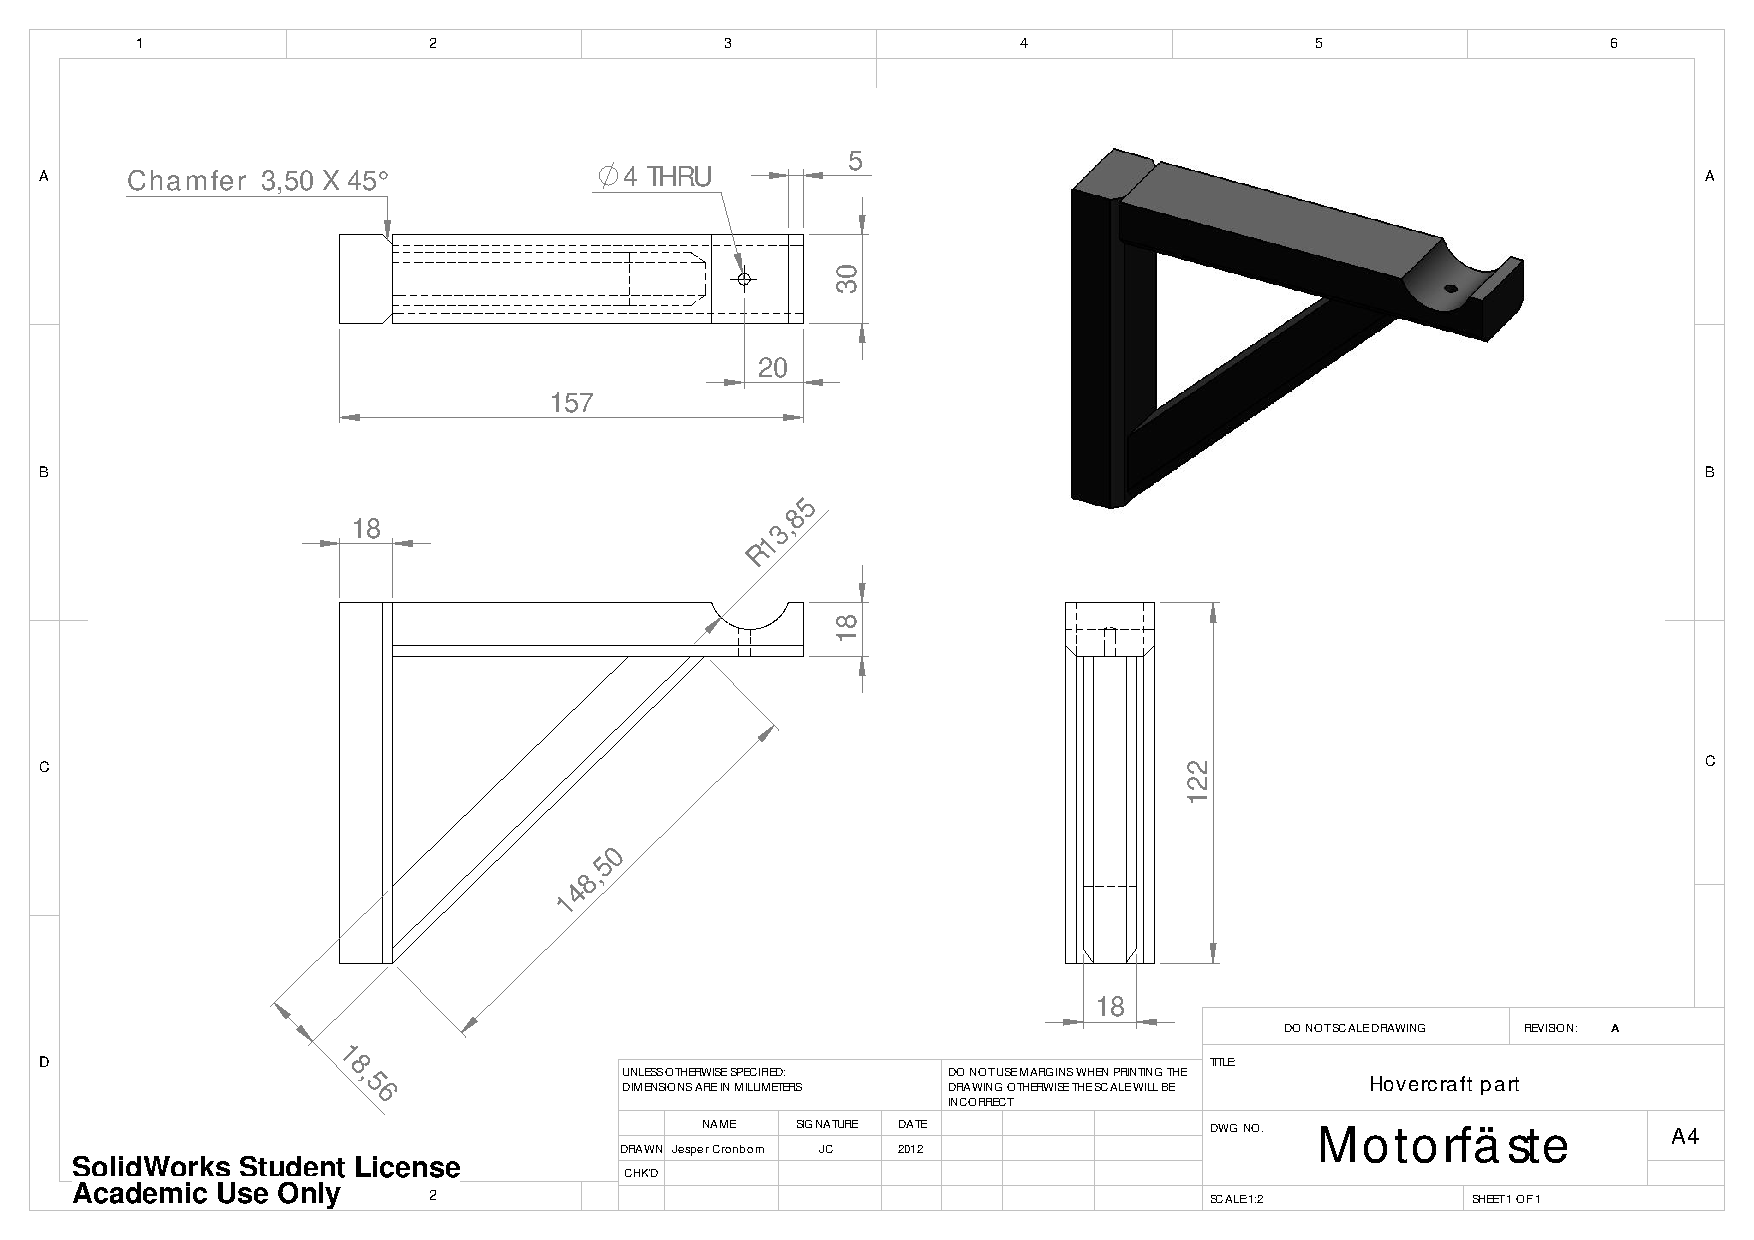
\includegraphics[width=18cm]{../../includes/figures/PDF_ritningar/Motorfaste}
\caption{Ritning över motorfäste.}
\label{fig:motorfaste}
\end{figure}
\end{landscape}

\begin{landscape}
\begin{figure}[htbp!]
\centering
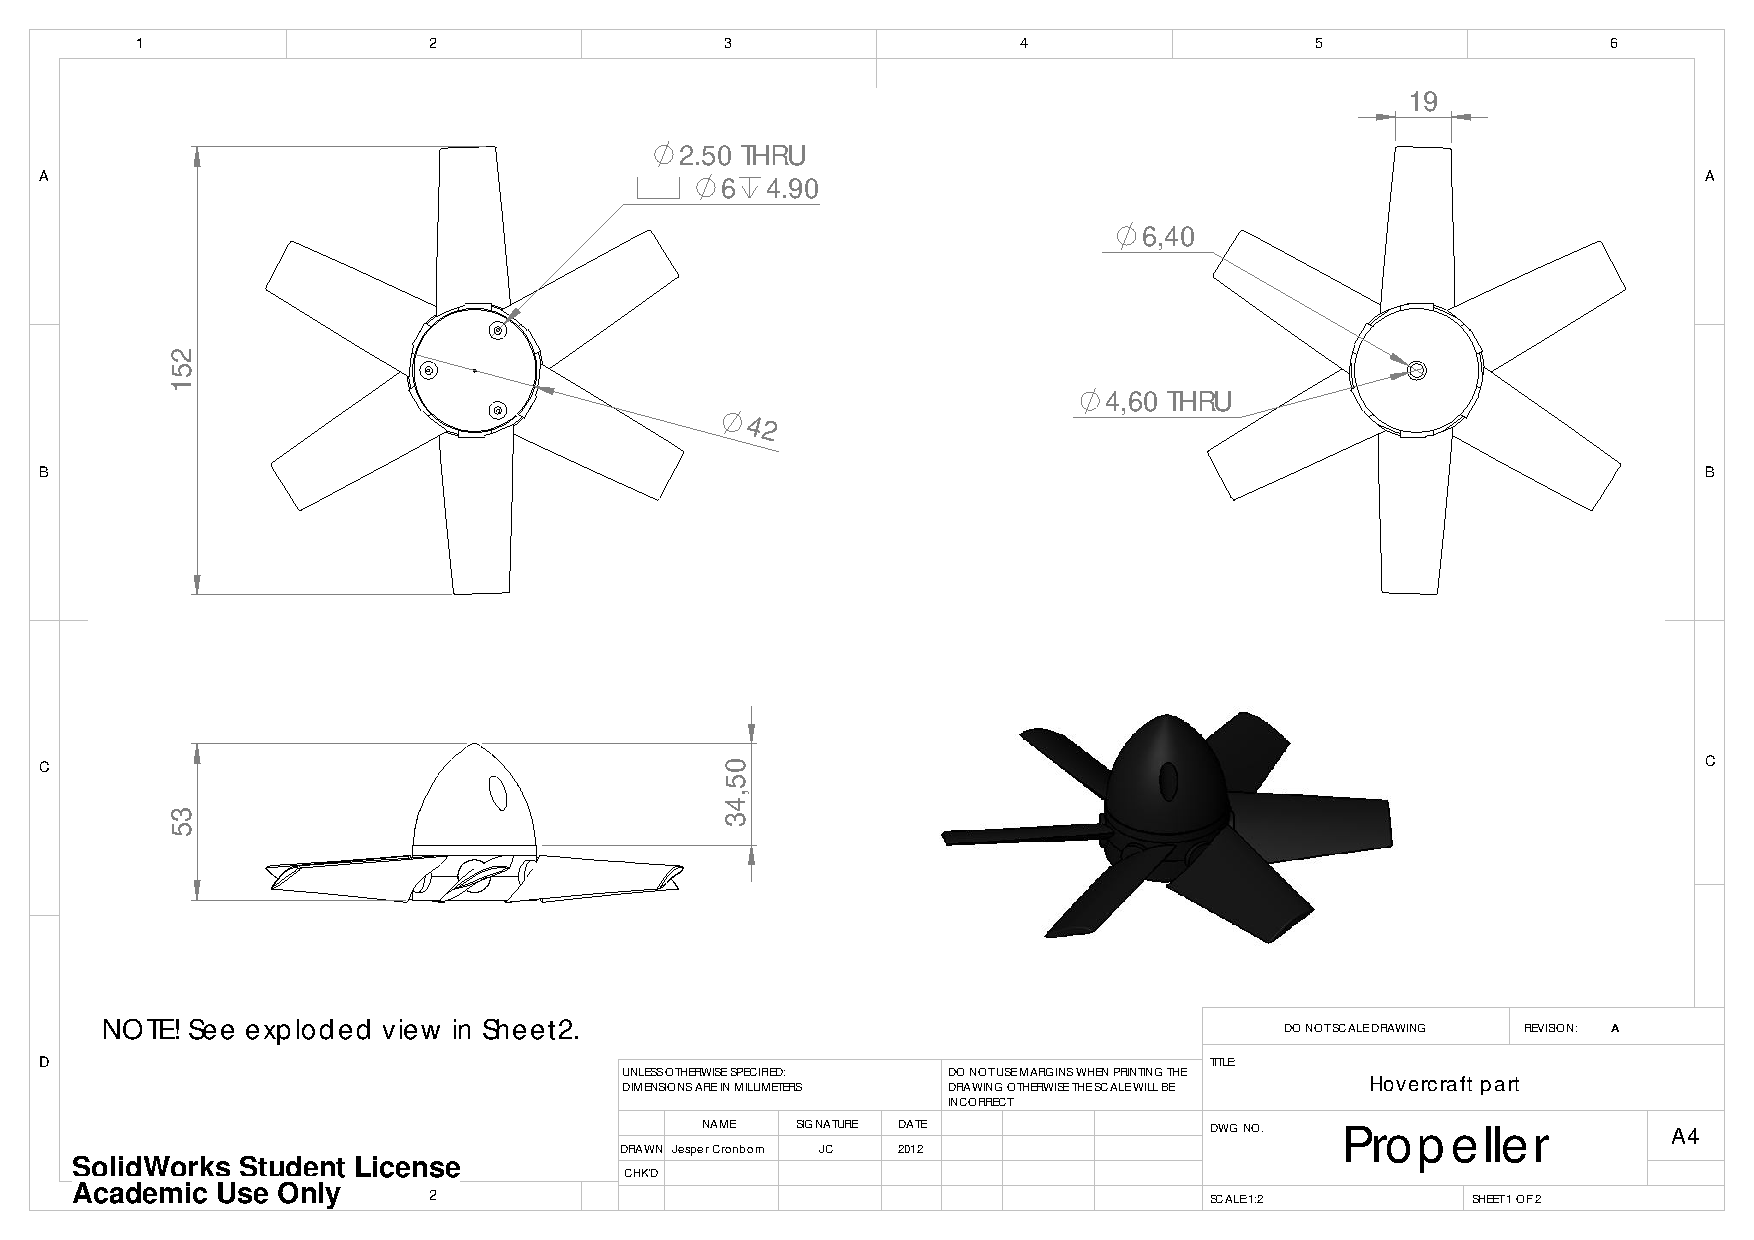
\includegraphics[width=18cm]{../../includes/figures/PDF_ritningar/Propeller}
\caption{Ritning över propeller.}
\label{fig:propeller}
\end{figure}
\end{landscape}

\begin{landscape}
\begin{figure}[htbp!]
\centering
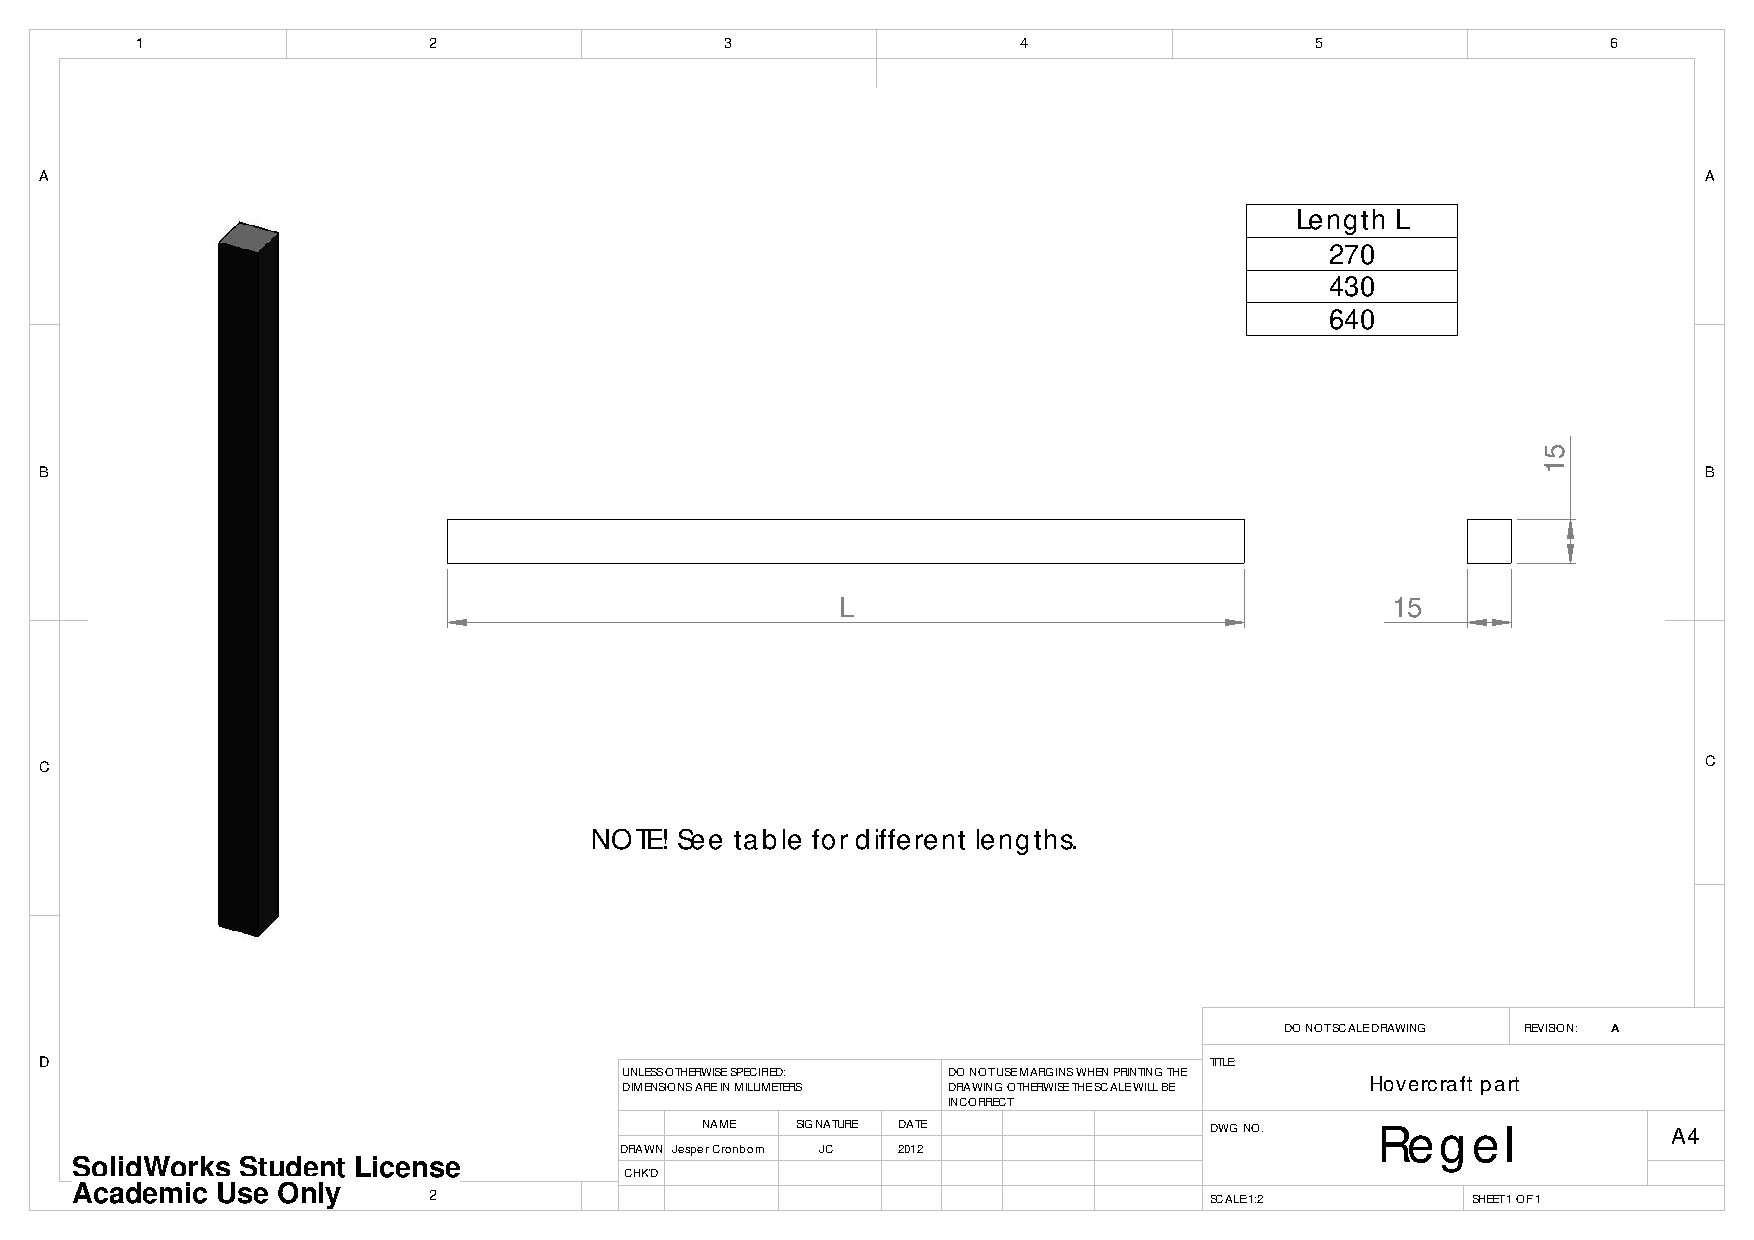
\includegraphics[width=18cm]{../../includes/figures/PDF_ritningar/Regel}
\caption{Ritning över regel.}
\label{fig:regel}
\end{figure}
\end{landscape}

\begin{landscape}
\begin{figure}[htbp!]
\centering
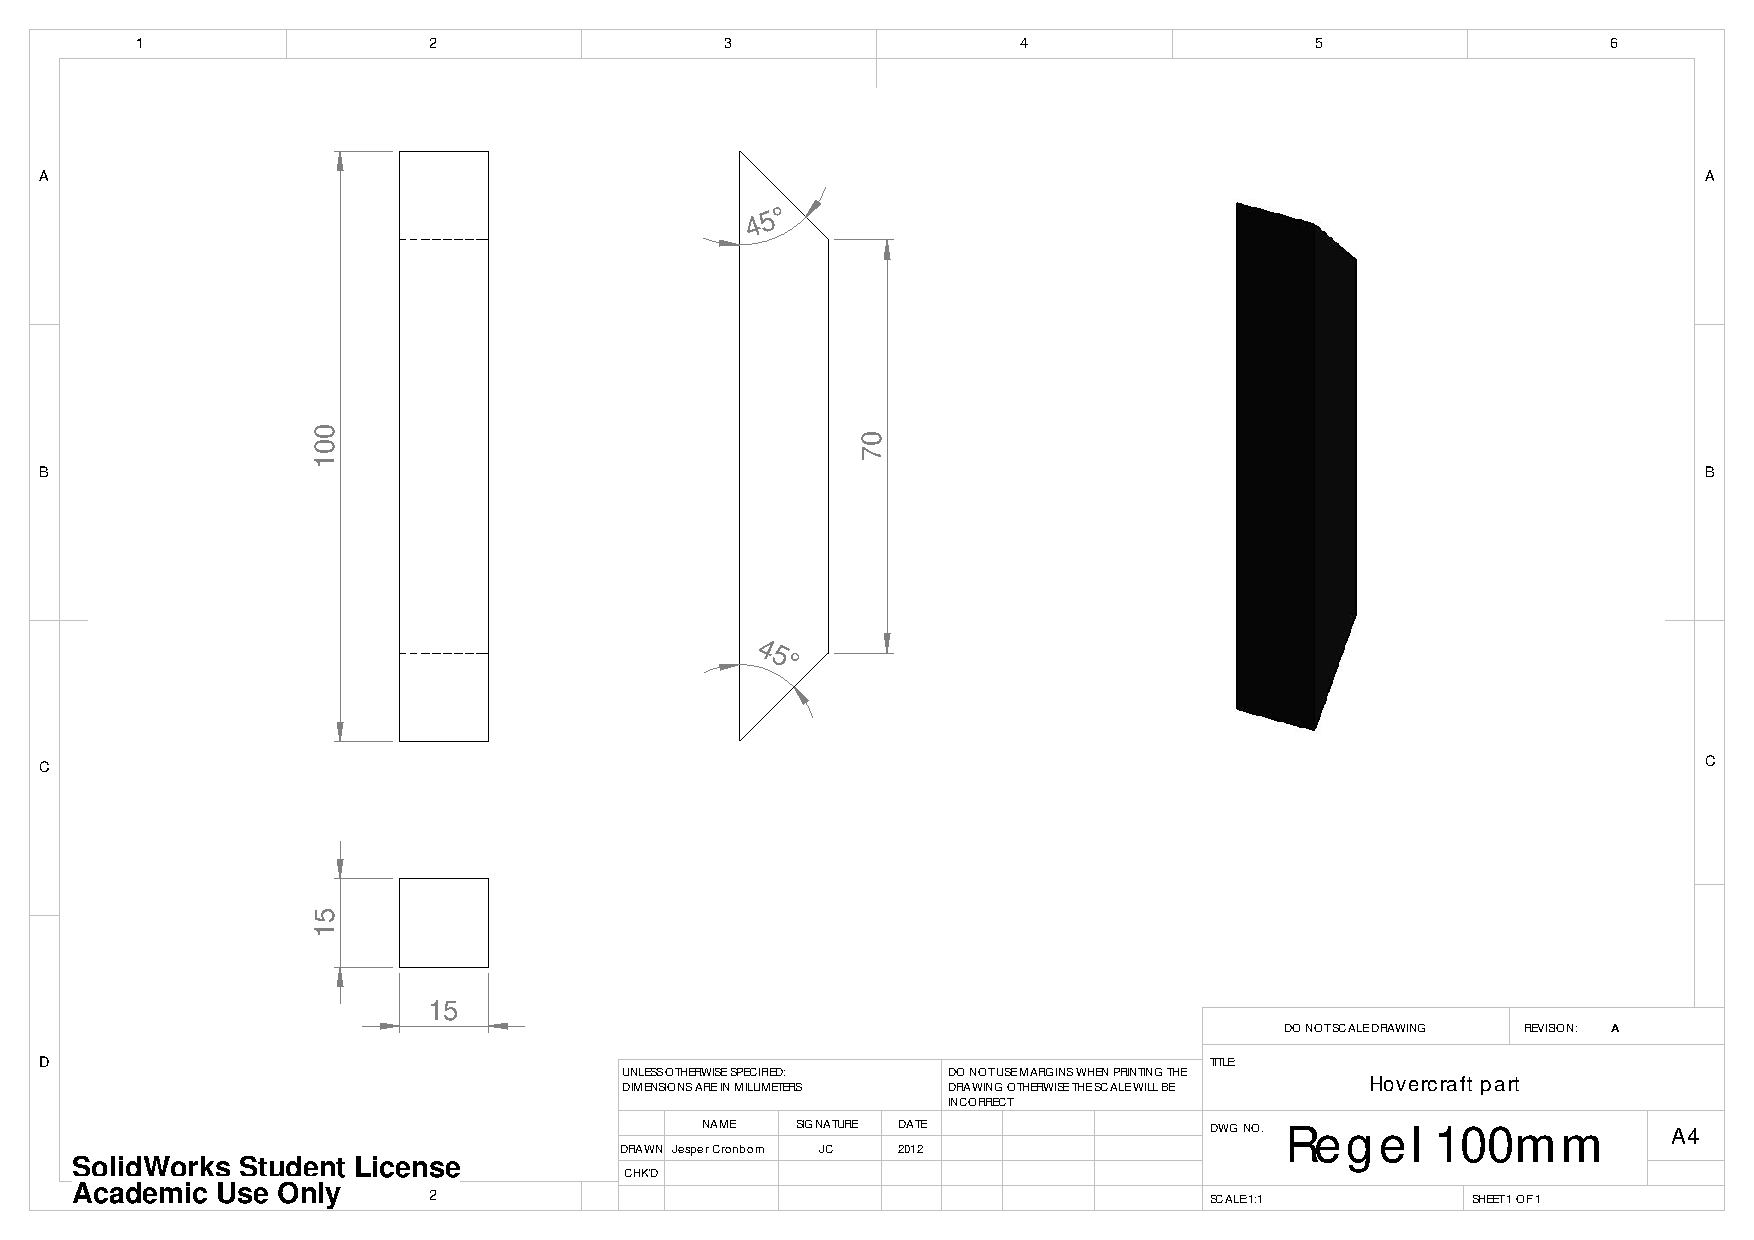
\includegraphics[width=18cm]{../../includes/figures/PDF_ritningar/Regel_100}
\caption{Ritning över regel 100.}
\label{fig:regel_100}
\end{figure}
\end{landscape}

\begin{landscape}
\begin{figure}[htbp!]
\centering
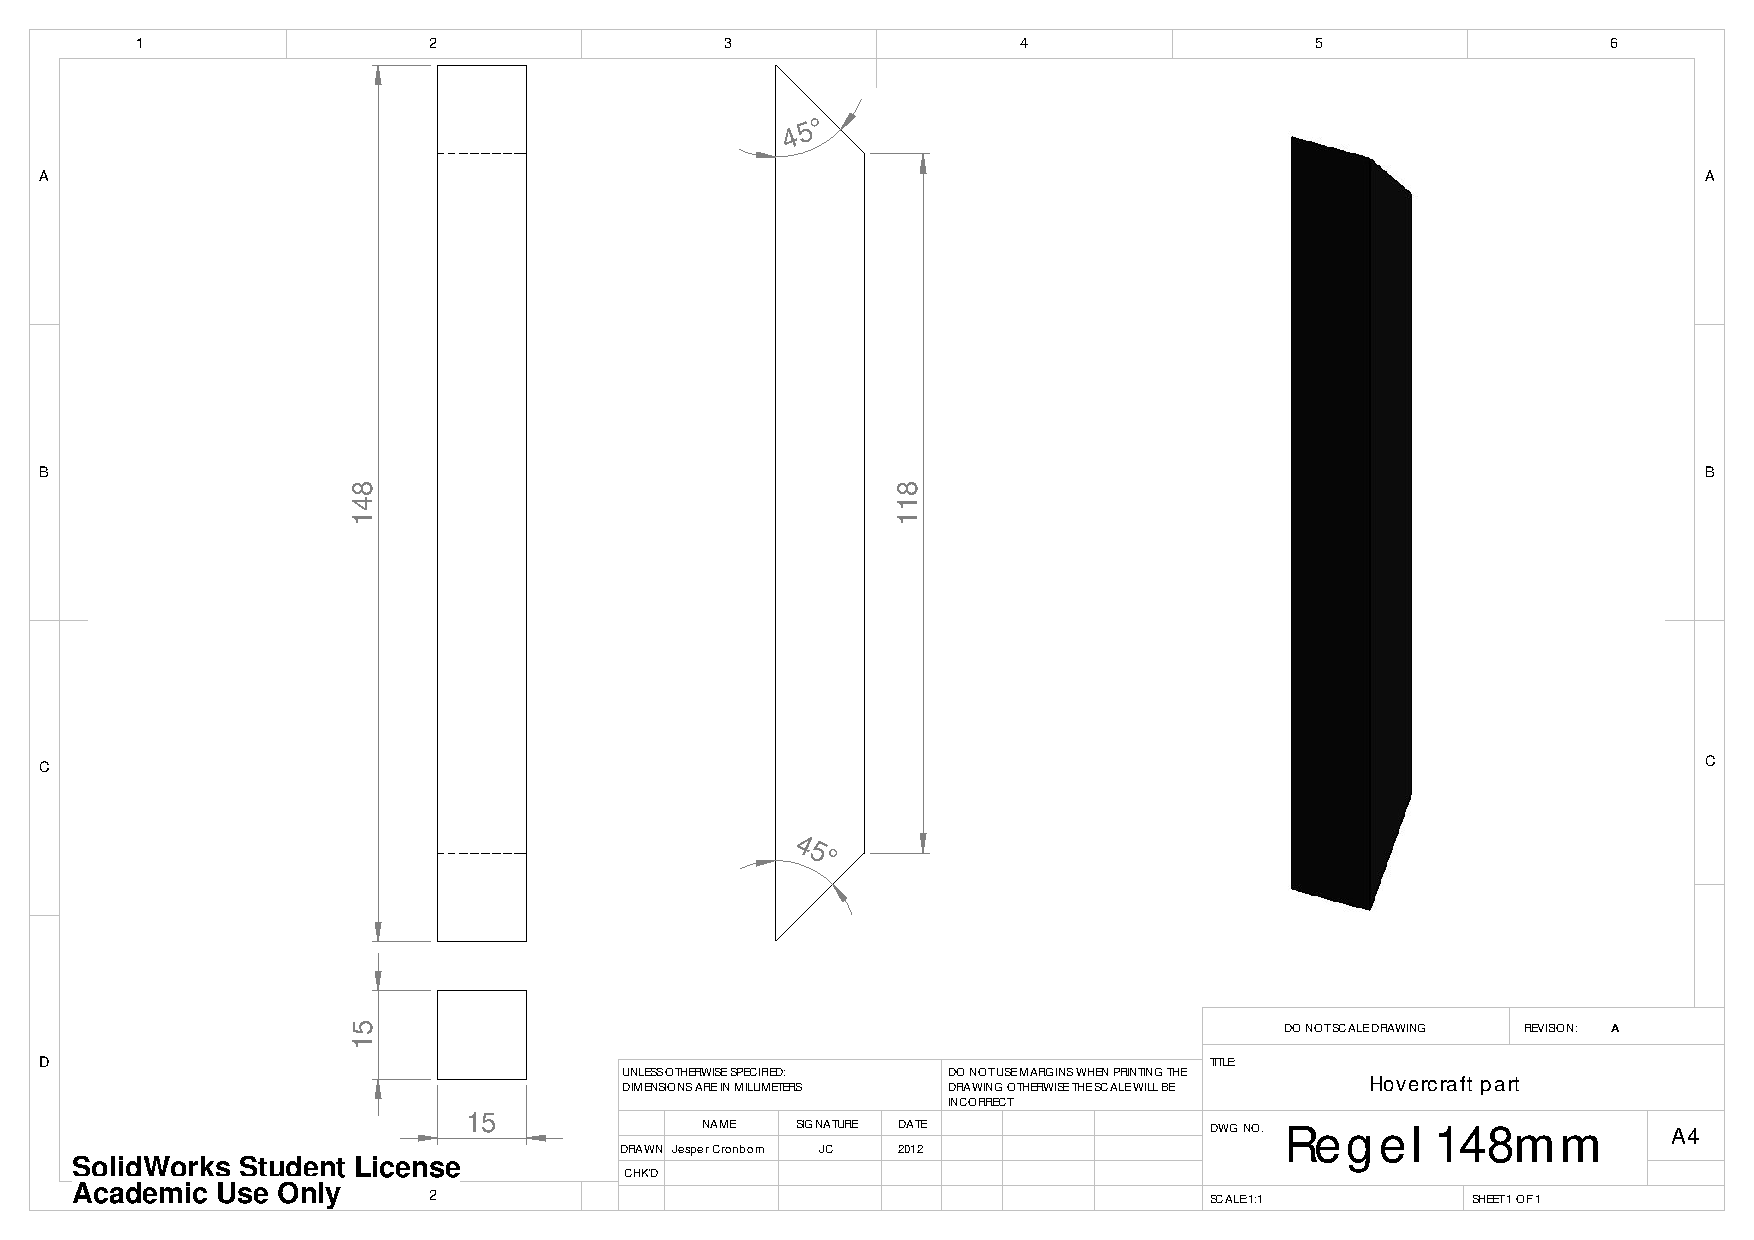
\includegraphics[width=18cm]{../../includes/figures/PDF_ritningar/Regel_148}
\caption{Ritning över regel 148.}
\label{fig:regel_148}
\end{figure}
\end{landscape}

\begin{landscape}
\begin{figure}[htbp!]
\centering
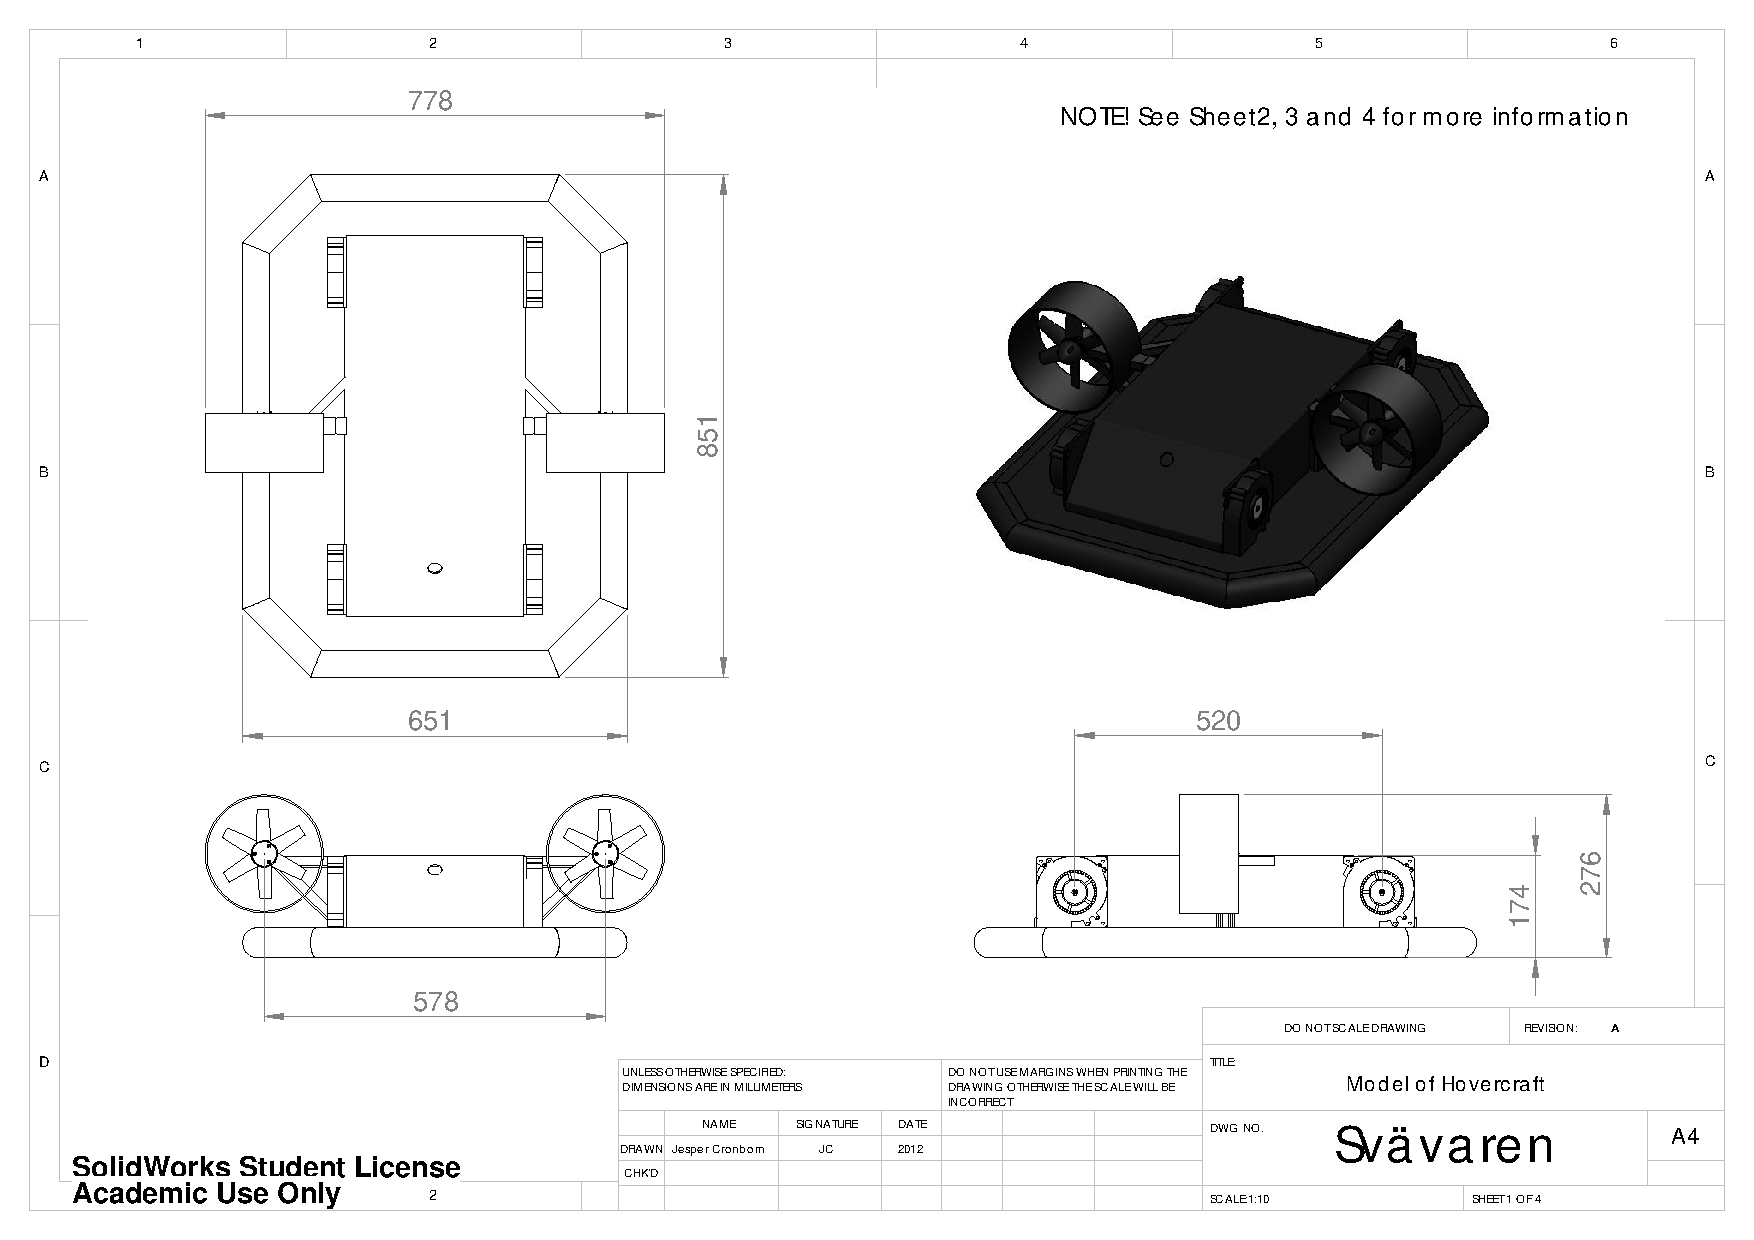
\includegraphics[width=18cm]{../../includes/figures/PDF_ritningar/Svavaren}
\caption{Ritning över svävaren.}
\label{fig:Svavaren_full}
\end{figure}
\end{landscape}

\begin{landscape}
\begin{figure}[htbp!]
\centering
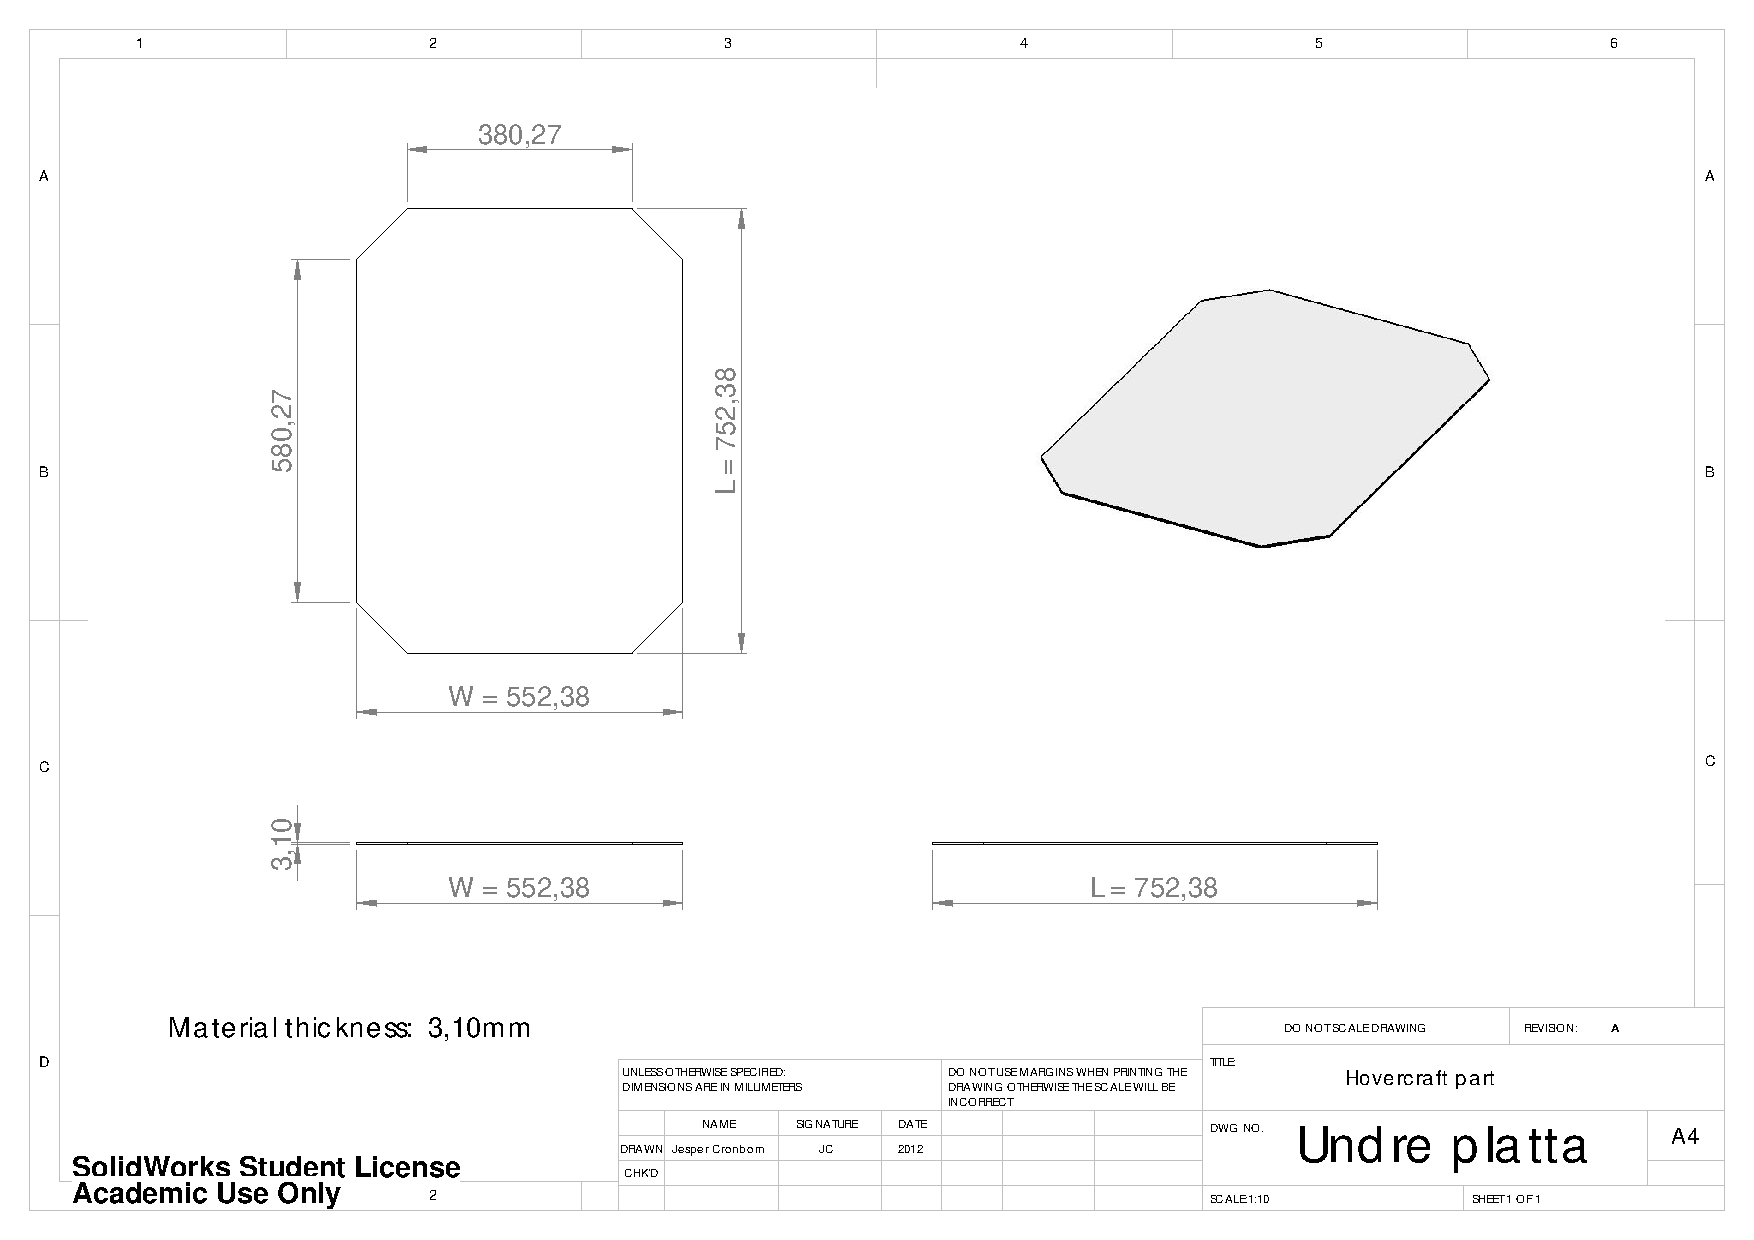
\includegraphics[width=18cm]{../../includes/figures/PDF_ritningar/Undre_platta}
\caption{Ritning över svävaren.}
\label{fig:Svavaren}
\end{figure}
\end{landscape}

\begin{landscape}
\begin{figure}[htbp!]
\centering
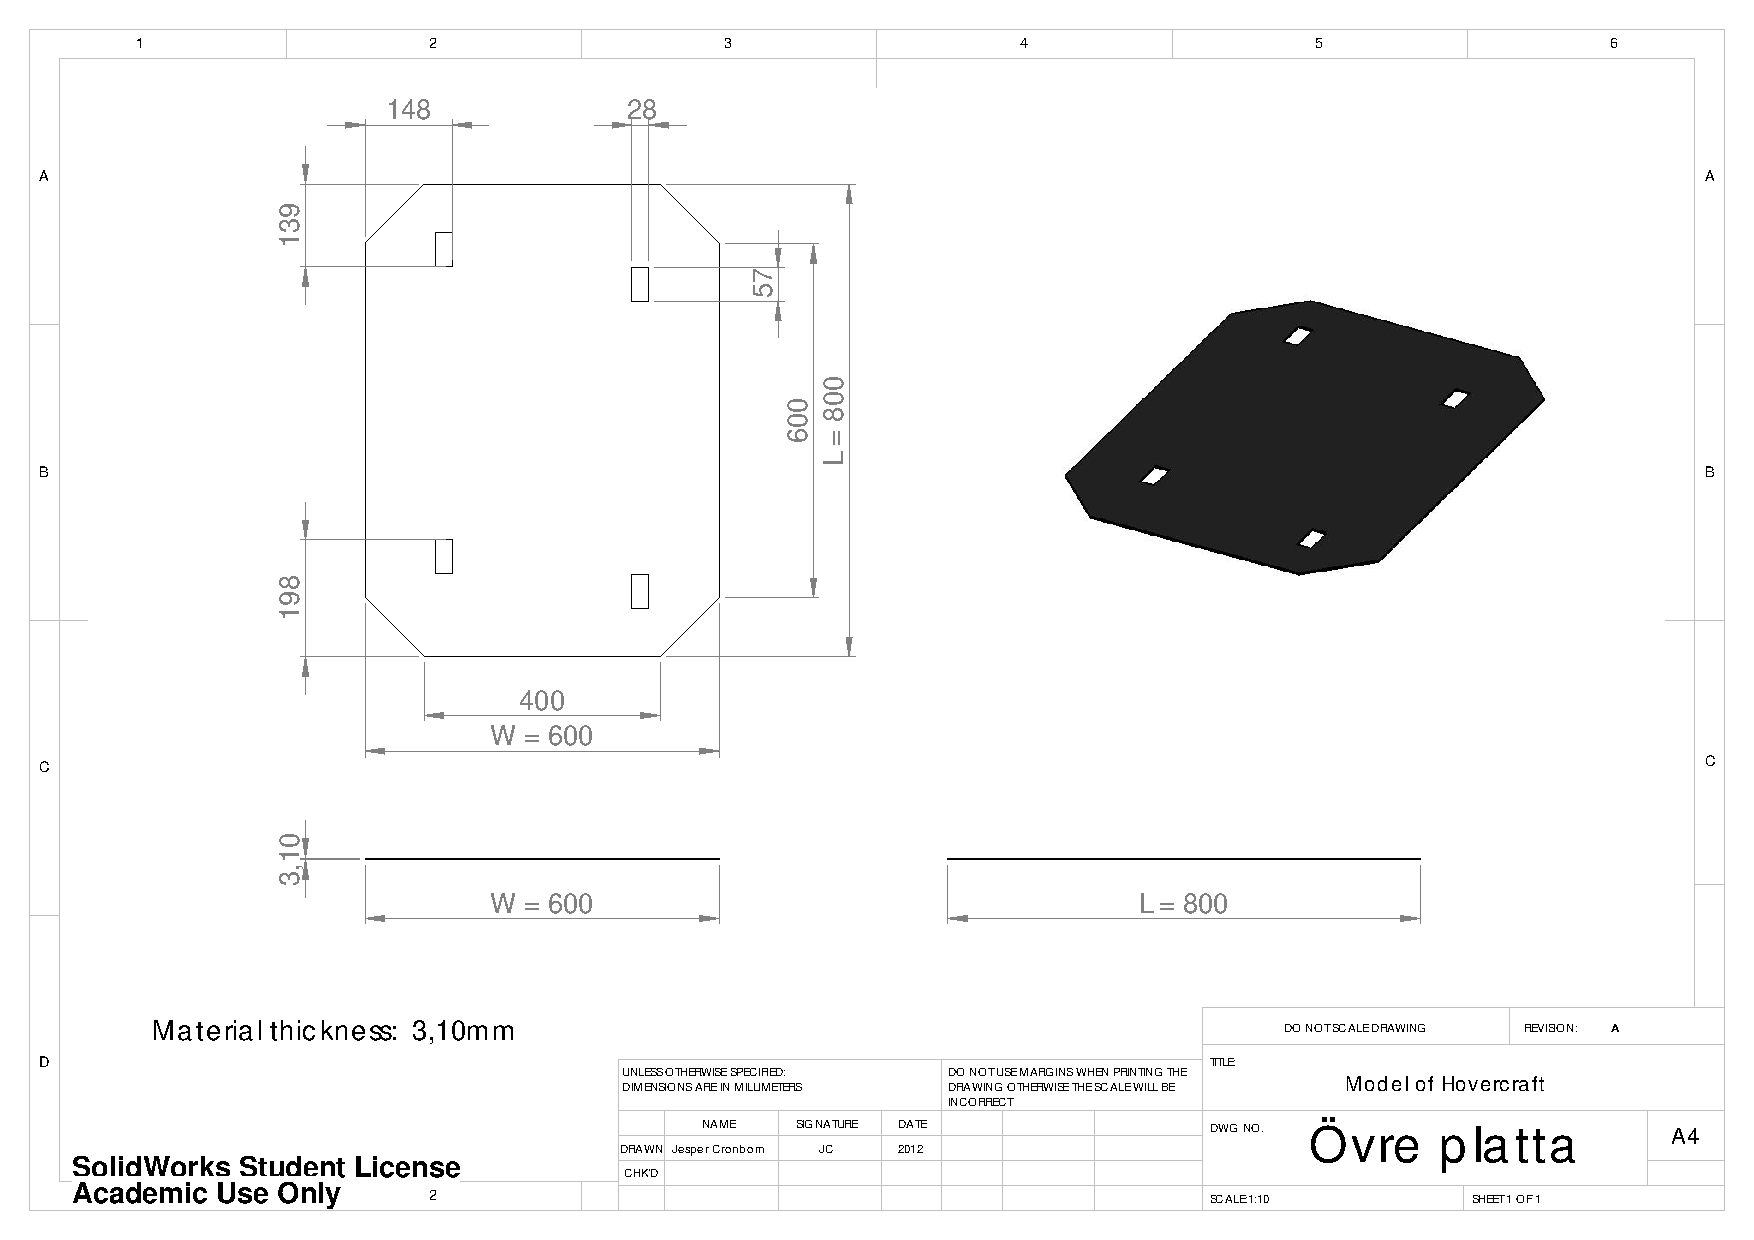
\includegraphics[width=18cm]{../../includes/figures/PDF_ritningar/Ovre_platta}
\caption{Ritning över övre plattan.}
\label{fig:Ovre_platta}
\end{figure}
\end{landscape}



\newpage
\section{Rapport H-brygga}
\label{apx:H-bridge}
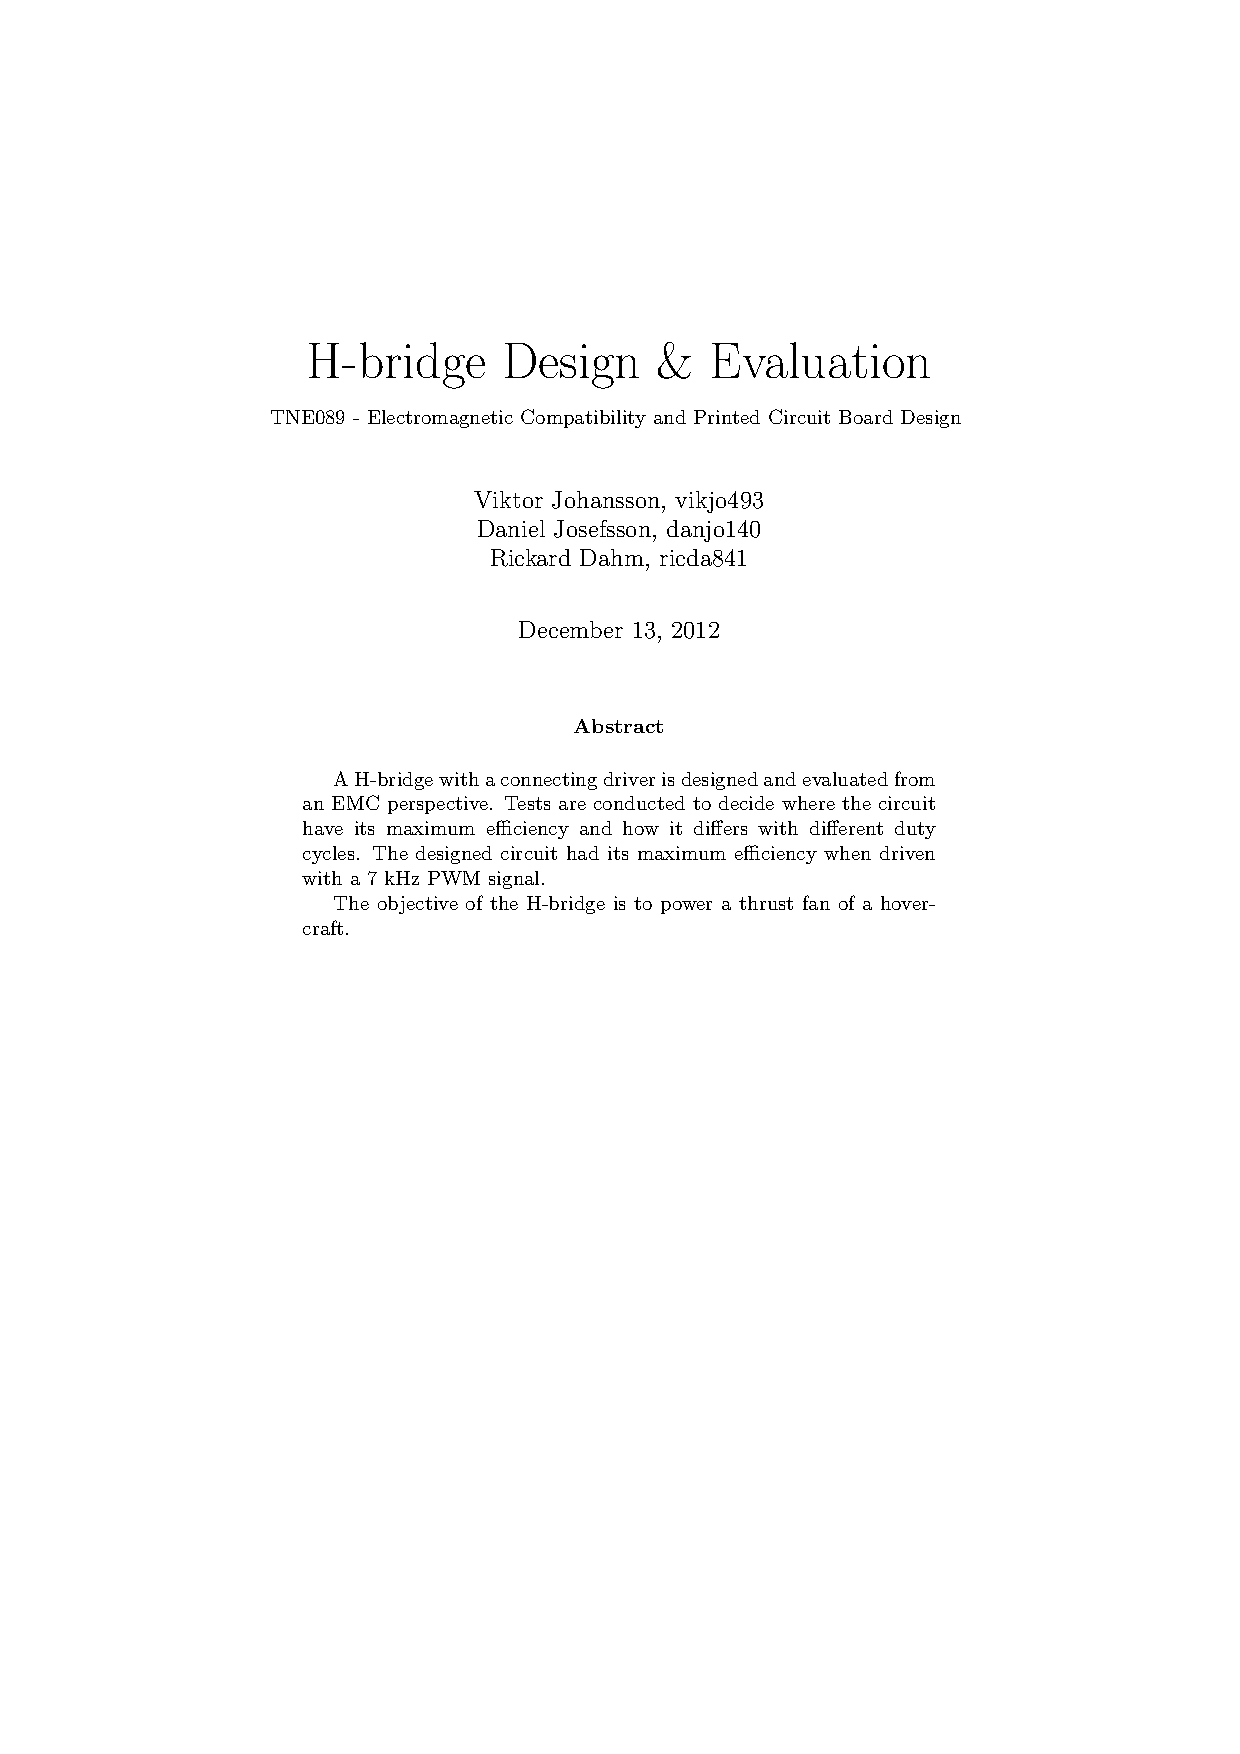
\includepdf[pages={-}]{appendix/TNE089-Project_Report_h_birdge.pdf}

\section{Rapport strömförsörjning}
\label{apx:PSU}

\includepdf[pages={-}]{appendix/TNE089-PowerSupplyReport.pdf}
